\documentclass[12pt, oneside]{report}

\usepackage[utf8]{inputenc}
\usepackage[
    style=authoryear,
    defernumbers=true,
    backend=biber,
    dashed=false,
    maxnames=999,
    maxcitenames=3,
    giveninits=true,
    urldate=long,
    uniquename=false,
    uniquelist=false
]{biblatex}

%\includeonly{lectures/lecture17}

\usepackage{IEEEtrantools}
\usepackage[margin=.85in]{geometry}
\usepackage{graphicx}
\usepackage{mathptmx}
\usepackage{xcolor}

\usepackage[
    colorlinks=false,
    linkbordercolor=white,
    citebordercolor=white,
    filebordercolor=white,
    urlbordercolor=white
]{hyperref}

\addbibresource{references.bib}

\usepackage{subcaption}
\usepackage{amsthm}
\usepackage{amsmath}
\usepackage{enumitem}

%\usepackage[utf8]{inputenc}
\usepackage[T1]{fontenc}
\usepackage{tabularx}
\usepackage{titlesec}

\linespread{1.25}
\pagestyle{plain}

\newtheorem{theorem}{Theorem}
\newtheorem{definition}{Definition}
\newtheorem{lemma}{Lemma}
\newtheorem{Rule}{Rule}

\numberwithin{definition}{chapter}
\numberwithin{theorem}{chapter}
\numberwithin{lemma}{chapter}
\numberwithin{Rule}{chapter}
\numberwithin{equation}{chapter}

\titlespacing{\chapter}{0pt}{*4}{*2.5}
\titleformat{\chapter}{\normalfont\huge\bf}{\thechapter}{20pt}{\huge\bf}

\setcounter{tocdepth}{1}


\begin{document}

\begin{titlepage}
    \begin{center}
        \vspace*{2cm}
        
        \LARGE
        Scientific and Large Data Visualization - class notes
        
        \vspace{0.5cm}

        
        \vspace{1.5cm}
        by Jingrui Zhu
   		  \vspace{1.5cm}
        
       
        \vfill
                
        \vspace{0.8cm}
        University of Pisa\\
        {a.a. 2025/2026}
        
    \end{center}
\end{titlepage}

\tableofcontents 
\addtocontents{toc}{~\hfill\textbf{Page}\par} 

\begin{abstract}
    Disclaimer: These personal notes are intended for educational purposes only and may contain errors or inaccuracies. 
    They are not a substitute for attending lectures, reading textbooks, or consulting with instructors. 
    The content is based on the author's understanding of the course material and may not reflect the official curriculum or the views of the instructor. 
\end{abstract}

\chapter{Lecture 1 - Introduction}
The course is held by external lecturers, Prof.ssa \textit{Daniela Giorgi} and Prof. \textit{Massimiliano Corsini}.\par
The exam is of 2 parts, a visualization \emph{project} agreed upon with lecturers and an \emph{oral} examination on the notions and concepts presented during the course.\par
The \textbf{main objective} of the course is to learn \textit{how to create an appropriate visualization} for the data we have by learning how to transform data into a graphical representation and when to use different kind of visual representations.

\section{Introduction}
In \textit{scientific visualization}, there is a natural relationship between what is represented and its visual representation, whereas in \textit{information visualization}, the relationship is conventional, and it is up to designer to decide on the best representation. \par
The goal is to transform data to make sense out ot it. 
\subsection{Information visualization}
There are different perspectives to view the information visualization, either as applied science or as a technology.\par
Information visualization as an \textbf{applied science} is that a value of a good visualization let us see patterns in data, and therefore the science of pattern perception can provide a basis for design decisions.\par

Information visualization as a \textbf{technology} is a tool for communication for the understanding and the analysis. The functional constraints from the design of a technological object must depend on the task it should help with, and the graphics form should be constrained by the function of the presentation.\par
\subsection{Why information visualization?}
Human are a visual species. The human visual system is very good at identifying and analyzing patterns. Visualizations are like cognitive artifacts, the tools that help humans to think better, like an abacus. \par
Visualization has to do with distributed cognition. Human cognitive system is made of our brain, mind, and sensors, but also of the environment around us, which we use to store and manipulate information.\par
Visualizations enable parallel processing of information, instead of sequential.\par
Explanatory visualizations are tools to present information, communicate data and messages, and explain something to somebody else. They are tools for readers to analyze what is being presented to them, and very often, the output of the exploratory analysis generates new questions.\par
\begin{figure}[htbp]
    \centering
    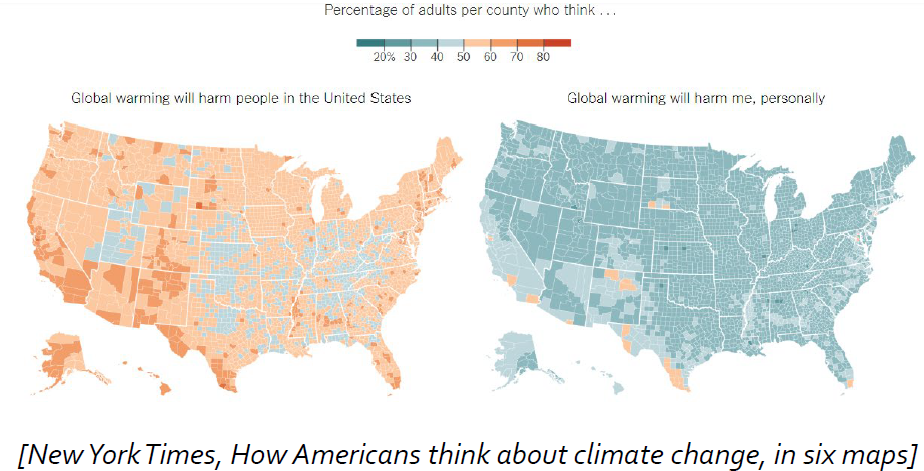
\includegraphics[width=0.5\linewidth]{imgs/lecture1/1.1 explanatory visualization.png}
    \caption{How visualizations convey messages}
    \label{fig:1.1}
\end{figure}
In confirmatory analysis, the reader has an hypothesis, and uses the visualization to see whether their hypothesis is true or not.\par

\subsection{Scientific visualization}
Scientific visualization are computing technique for the generation of interactive visual representations of acquired or simulated spatio-temporal data.\par
Data in ever-increasing sizes makes a graphical approach necessary. The modern process of visualization consists of taking raw data acquired through sensors or produced by some simulation and converting it to a form that is viewable and understandable to humans. \par

They also help us in identifying patterns and interpreting data, either simulated or acquired data. This can find applications in different fields, engineering, medicine, science, biology,...\par



\chapter{Lecture 2 - Basics}
\section{Why visualization}
Computer-based visualization systems provide visual representations of datasets designed to help people carry on tasks more efficiently.\par
Visualization allows people to analyze data when they do not know exactly what questions they need to ask in advance. Otherwise, they can use computational techniques from statistics or learning. \par
If there are many possible questions to ask, the best path forward is an analysis process with a \emph{human in the loop}, with a visual system augmenting human capabilities, rather than replacing it.\par
Visualization allows people to offload internal cognition and memory usage to the perceptual system, using images as external representations. \par
Visualization exploits the human visual system as a mean of communication. A significant amount of visual information process occurs in parallel at the preconscious level. \par
\begin{figure}[htbp]
    \centering
    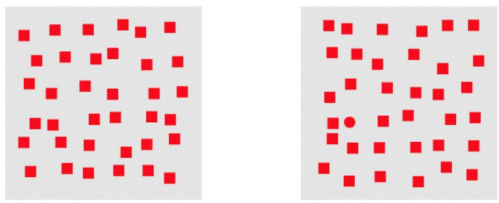
\includegraphics[width=0.3\linewidth]{imgs/lecture2/2.1 dependence on visual.png}
    \caption{Dependence on vision}
    \label{fig:2.1}
\end{figure}
Human vision can quickly find out the odd one in the fig~\ref{fig:2.1}, unlike other senses, because of the lack of parallelism in information processing.\par
\subsection{Visualization tools}
Visualization tools help people in situations where seeing the dataset structure in detail is better than seeing only a brief summary of it. \par
As the fig~\ref{fig:2.2} displays, by transforming numeric data into graphics, we can see how the data values change according to the X and Y.\par
\begin{figure}[htbp]
    \centering

    \begin{subfigure}[b]{0.32\linewidth}
        \centering
        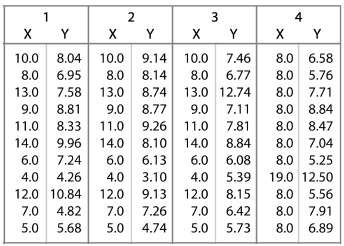
\includegraphics[width=\linewidth]{imgs/lecture2/2.2 visualization in summary.png}
        \caption{Table summary}
        \label{fig:2.2a}
    \end{subfigure}
    \hfill
    \begin{subfigure}[b]{0.32\linewidth}
        \centering
        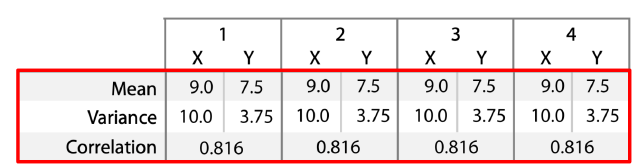
\includegraphics[width=\linewidth]{imgs/lecture2/2.3 visualizztion in detail.png}
        \caption{Table details}
        \label{fig:2.2b}
    \end{subfigure}
    \hfill
    \begin{subfigure}[b]{0.32\linewidth}
        \centering
        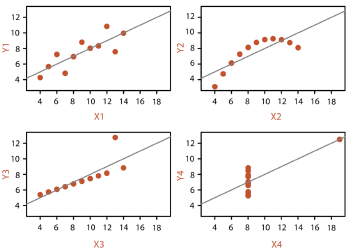
\includegraphics[width=\linewidth]{imgs/lecture2/2.4 visualization matters.png}
        \caption{Table data in graph}
        \label{fig:2.2c}
    \end{subfigure}

    \caption{Why visualization tools matter}
    \label{fig:2.2}
\end{figure}

\subsubsection{Interactivity}
Sometimes, the quantity of data is immense, and the limitations of both people and displays preclude showing everything at once. With interaction, user actions can change the view and investigate at multiple levels of detail. Look at an interactive map service, like GoogleMaps.\par

\subsubsection{Limitations}
Visualizations have limitations, especially when they come from "hardware" limitations. Human limitations are the finite resources for memory and attention. Computational capacity renders scalability a concern. And also, how the information is displayed.

\subsubsection{Task focused}
The user task is an important constraint on the visualization, as much as the data itself. \par
Visualization tools can support presentation, discovery, enjoyment of information, or even production of more information for subsequent use. A suitable visualization tool for one task is not necessarily fit for another task on the same dataset (No free lunch). Therefore, we must learn to understand which kind of visual representation to use, depending on both data and task.\par

\subsubsection{Effectiveness}
The focus on effectiveness is a corollary of defining visualization to have the goal of supporting user tasks. The goal of the designer is not to make pleasing figures but to render the results effective.\par
The vast majority of the possibilities in the design space can be ineffective in a specific usage context. This can be caused by poor design match with the properties of the human perceptual and cognitive system, or maybe it is a poor match with the intended task. 

\section{What-Why-How}
The What-Why-How method for visualization design is to answer the questions when designing the visualization.\par
\emph{What} data is being visualized? \emph{What} data are shown in the views?\par
\emph{Why} does the user need a visualization? \emph{Which} is the task being performed? \par
\emph{How} is the visual idiom constructed in terms of design choices?\par


\subsection{Semantics}
The data semantics refers to the real-world meaning of the data. As it should be provided for each dataset, as metadata. For example, the word "Apple" refers to what, the company? The fruit? the city? By means of semantics, we can take care of the ambiguity behind the data.

\section{Data Type}
The type of data is its mathematical or structural interpretation. 
There are five basic data types in visualization:
\begin{itemize}[noitemsep]
    \item \emph{Items}: an individual entity that are discrete in the dataset. They can be seen as a row in a table. 
    \item \emph{Attributes}: some specific property that can be measured, observed, or logged. In practice, they are properties of objects, also called as variables
    \item \emph{Links}: a relationship between items, typically within a network.
    \item \emph{Positions}: 2D or 3D spatial data (latitude and longitude)
    \item \emph{Grids}: they specify the strategy for sampling continuous data in terms of both geometric and topological relationships between its cells
\end{itemize}

\section{Attribute type}
The major distinction between attribute types is \emph{categorical vs ordered}. \par
\emph{Categorical} attributes are attributes whose values describe categories and do not have an implicit ordering. They can have an imposed external ordering (alphabetical order, for instance), but it is not intrinsic to the attribute itself. \par
\emph{Ordered} attributes have an implicit ordering.\par
One must choose an appropriate visual representation according to the attribute types and semantics

\subsection{Ordered attributes}
Ordered attributes can be further subdivided into:
\begin{itemize}[noitemsep]
    \item \textbf{Ordinal}: attributes which have a well-defined ordering but do not support full-pledged arithmetics (shirt size, ranking, etc.)
    \item \textbf{Quantitative}: attributes whose values represent measured quantities/magnitudes and that support arithmetic comparison (temperature, height, price, etc.)
\end{itemize}\par

Ordered attributes can have different semantics:
\begin{itemize}[noitemsep]
    \item \textbf{Sequential}: there is a homogeneous range from a minimum to a maximum value (height).
    \item \textbf{Diverging}: there are 2 sequences pointing in opposite directions that meet at a common zero-point (temperature has positive/negative value ranges).
    \item \textbf{Cyclic}: the values are wrapped around back to a starting point (hours of a day)
\end{itemize}
\section{Dataset types}
A dataset is a collection of information that is the target of analysis. The 4 basic dataset types are \emph{tables, networks, fields, and geometry}. Each of them arise from combinations of the data types of items, attributes, links, positions, and grids.\par
\begin{figure}[htbp]
    \centering
    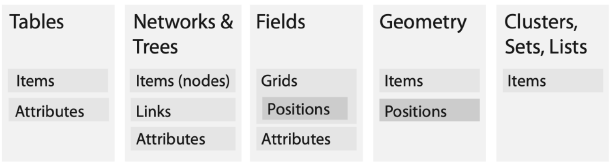
\includegraphics[width=0.5\linewidth]{imgs/lecture2/2.8 dataset types.png}
    \caption{Data and Dataset type combinations}
    \label{fig:2.6}
\end{figure}

\subsubsection{Tables}
Many datasets come in the form of tables of rows and columns, like in a spreadsheet. In a flat table, each row represents an item, and each column is an attribute of the dataset. Each cell contains a value for that pair. Multi-dimensional tables have slices and multiple keys.

\subsubsection{Networks}
Networks are suitable to specify that there is some kind of relationship between two or more items. An item in a network is called a node, and a link between 2 nodes is a relationship between two items. A network node and link can have attributes associated with them. 

\subsubsection{Trees}
Trees are networks with a hierarchical structure and no cycles. Each child node has exactly one parent node pointed to it. \par
A tree is a typical representation for hierarchy, like the organization chart of a company, or an evolutionary relationship between species in the biological tree of life.

\subsubsection{Meshes}
A 3D mesh is a particular type of graph used in computer graphics to represent 3D models. Nodes are called vertices, arcs are called edges, and there are also polygons called faces.

\subsubsection{Geometry}
They specify information about the shape of items with explicit spatial positions. 

\subsection{Fields}
Fields are a type of dataset in which values associated with a cell contain measurements or calculations from a continuous domain. Since we have a continuous domain, fields require \emph{sampling}, the measurement frequency, and \emph{interpolation}, how to show values in between the sampled points. \par
Field values are stored in grids, which have 2 properties:

\begin{itemize}[noitemsep]
    \item Geometry: position of cells in space
    \item Topology: the way cells are connected to adjacent ones
\end{itemize}

According to the values stored in cells, we can distinguish among scalar fields, vector fields, and tensor fields. These values can be static or time-dependent; deterministic or uncertain. \par

\begin{itemize}[noitemsep]
    \item \emph{Scalar} fields is one in which each cell contains a single value, for example, gray level values in medical imaging
    \item \emph{Vector} fields are ones where each cell contains a vector, represented as direction and modules (for instance, velocity)
    \item \emph{Tensor} fields are the ones where each cell contains a multi-dimensional array of attributes at each point
\end{itemize}

Continuous data is often found in the form of a spatial field, where the cell structure of the field is based on sampling at spatial positions. The data contain information about both sampled values and the position where they have been acquired.\par
According to grid geometry and grid topology, we have different types of grids: \emph{uniform, rectilinear, structured, unstructured}.

\subsubsection{Uniform grid}
They sample at a regular interval; there is no need to explicitly store topology. A uniform grid is formed of tessellations of the Euclidean plane/space by square/cubic elements, points are spaced regularly along each direction.

\subsubsection{Rectilinear grid}
They support non-uniform sampling for an efficient storage of information, at the cost of having to store geometric locations. They are useful to adapt the sampling to the geometry of the data. Its tessellations are of rectangles/rectangular cuboids, regular grids, but the spacing of points along axes can vary. They are useful to adapt the sampling to the geometry of the data. It has a fixed connectivity, yet needs to store information for spacing.

\begin{figure}[htbp]
    \centering
    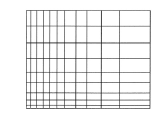
\includegraphics[width=0.2\linewidth]{imgs/lecture2/2.11 rectilinear grid.png}
    \caption{Rectilinear grid}
    \label{fig:2.9}
\end{figure}

\subsubsection{Structured grid}
They allow a curvilinear shape. It has the same connectivity as the previous two types, but an irregular geometry. Points can be replaced at an arbitrary coordinate, but no overlapping or self-intersections. It has to store the geometry of each cell.

\begin{figure}[htbp]
    \centering
    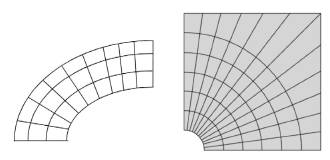
\includegraphics[width=0.2\linewidth]{imgs/lecture2/2.12 structured grid.png}
    \caption{Structured grid}
    \label{fig:2.10}
\end{figure}

\subsubsection{Unstructured grid}
They have complete flexibility, but need to store spatial positions and topological information about how the cells connect to each other. It allows different combinations of cells (a popular choice).

\begin{figure}[htbp]
    \centering
    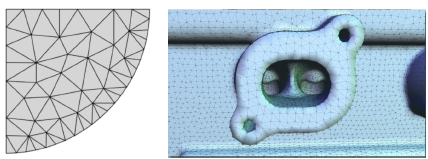
\includegraphics[width=0.25\linewidth]{imgs/lecture2/2.13 Unstructured grid.png}
    \caption{Unstructured grid}
    \label{fig:2.11}
\end{figure}

It can also be under the form of a cloud of points, but this does nor explicit any connectivity information and have irregular geometry.

\chapter{Lecture 3 - Basics}
\section{Visual encoding}
Visual encoding means \emph{going from data to visual representations}. Encoding requires not only choosing a graph that is appropriate for the data at hand (its type and semantics), but also selecting the individual graphical elements and their properties.\par
There are two core graphical elements in a visualization: visual marks and visual channels. \emph{Marks} are basic geometric/graphical elements that depict items or links (a point, a line, a polygon, ...). \emph{Channels} are visual properties that control the appearance of marks (color, dimension, ...) and depict attributes.\par
They are the building blocks for analyzing visual encoding; even complex visual encoding can be broken down into components that can be analyzed in terms of their marks and channel structure. The effectiveness of marks and channels for encoding data depends on data types.

\begin{definition}[Marks]
    A mark is a basic graphical element, a geometric primitive. They are classified according to the number of spatial dimensions they require: 
    \begin{itemize} [noitemsep]
        \item 0-dim: points
        \item 1-dim: line, segments
        \item 2-dim: areas
        \item 3-dim: volumes
    \end{itemize}
\end{definition}

\begin{definition}[Channels]
    Visual channels are a way to control the appearance of marks and encode information about attributes, independent of the dimensionality of marks. Some main channels are:
    \begin{itemize}[noitemsep]
        \item spatial position: aligned, unaligned, depth, region ...
        \item color: hue, saturation, luminosity
        \item shape and texture
        \item slop and angle
        \item size: length(1D), area(2D), volume(3D)
    \end{itemize}
\end{definition}

Channels can be divided into 2 different categories, according to the two different sensor modalities on the human perceptual system: identity and magnitude channels.\par
\textbf{Identity} channels give information about what something is or where it is, like \textit{shape, color}.\par
\textbf{Magnitude} channels tell us how much of something there is, the \textit{length, area, saturation, size, ...}

\begin{definition}[Context]
    A contextual component can make a visualization much easier to interpret, such as legends, labels, annotations, and also grids, axes, reference lines, etc.
\end{definition}

\paragraph{Bar chart}
Bar chart encodes 2 attributes, a \emph{quantitative} one represented on the y-axis and a \emph{categorical} one represented on the x-axis.\par
Its typical mark is a line (bars, 1D marks). Two channels, one for vertical spatial position for the quantitative attribute and one for horizontal spatial position for the categorical attribute.

\paragraph{Scatterplot}
A scatterplot can encode multiple attributes. Its main mark is points (circles, 0D marks). It can have different channels: \textit{one} for vertical spatial position along the y-axis to represent a quantitative attribute; \textit{one} for horizontal spatial position along the x-axis for the second quantitative attribute; \textit{a third channel} could be color to represent a quantitative or qualitative attribute; a forth channel is the area of the points.

\section{Visual decoding}
Visual decoding means deconstructing a visual representation into its major units, and identifying the graphical elements \textit{(what are the visual marks and channels?)} and the mapping rules, i.e., the information that the graphical elements represent \textit{(What data items do the marks represent? What attribute do the channels represent?)}. It is useful for evaluating and redesigning visualizations.\par

\section{Expressiveness and Effectiveness}
Channels are not equal: the same data attribute encoded with two different visual channels will result in different information content on the users' side, after it has passed through the perceptual and cognitive pathways of the human visual system. \par
The use of marks and channels in visual design should be guided by the principles of \textbf{expressiveness and effectiveness}. There is a ranking of channels according to the type of data that is being visually encoded. Once you have identified the most important pieces of information in your data, you have to ensure they are encoded with the highest-ranked channels.

\begin{definition}[The Expressiveness Principle]
    The visual encoding should express all of, and only, the information that is present in the dataset attributes. Do not represent information and relationships that are not in the data, especially, do not use any color or position when the data does not encode any information.
\end{definition}

\textit{Ordered data} should be shown so that our visual system perceives them as ordered, by using \textit{magnitude channels.}\par
\textit{Unordered data} shouldn't be shown in a way that perceptually implies an ordering that does not exist, use \textit{identity channels}.

\begin{definition}[The Effectiveness Principle]
    The importance of the attribute should match the salience of the channel, i.e., its noticeability. Relevant information should be prioritized, then encoded with the most effective/accurate channels to be most noticeable. Decreasingly important attributes can be matched with less effective channels.
\end{definition}

\section{Channel rankings}
The ranking shows how effective the channels are at conveying different types of attributes.
\begin{figure}[htbp]
    \centering
    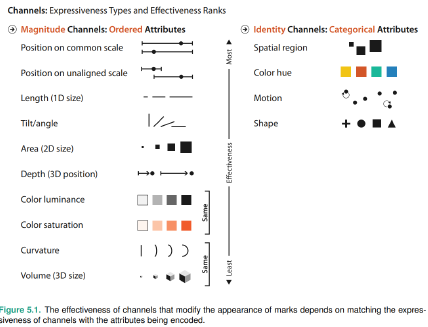
\includegraphics[width=\linewidth]{imgs/lecture3/3.4 channel rankings.png}
    \caption{A channel ranking}
    \label{fig:3.2}
\end{figure}

The fig~\ref{fig:3.4} shows one proposed channel ranking. As the figure shows, in both classifications, spatial channels appear at the top of the lists. The choice of which attributes to encode with position is the most central choice in visual encoding, as they will dominate a user's mental model.
\section{Visual representation, a counterexample}
\begin{figure}[htbp]
    \centering
    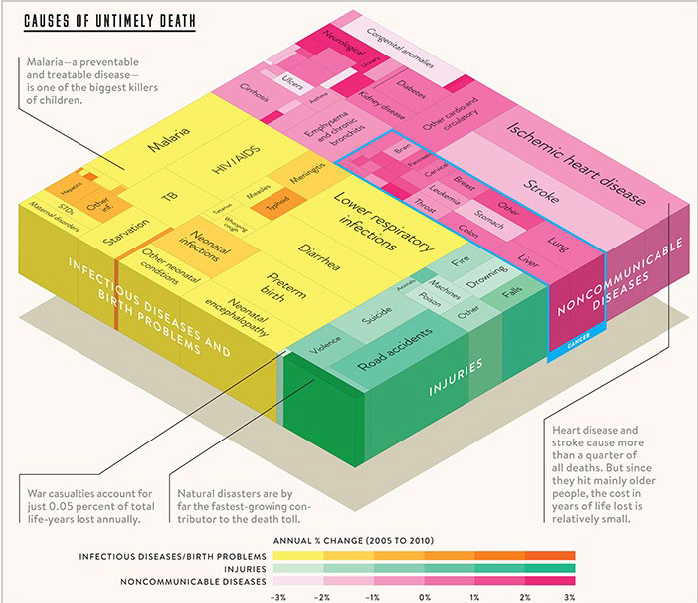
\includegraphics[width=0.5\linewidth]{imgs/lecture3/3.5 visual counterexample.png}
    \caption{A visual counterexample}
    \label{fig:3.5}
\end{figure}

The fig~\ref{fig:3.5} shows a visual representation of causes of death used in a debate. Where, each rectangle represents a death cause, the size of the rectangle represent years of life lost, the color represents the group of death, and the color intensity represents the change from one year to another.\par
It is a very complicated graph on a very complicated topic; some bad design choices made it less effective than it should be:
\begin{itemize}[noitemsep]
    \item the use of 3D projection is unnecessary, makes the perception of each rectangle much more difficult to comprehend.
    \item the area is not the best channel to represent quantities, also each rectangle has its own height and width, making the comparisons among causes much more difficult.
    \item Difficult in evaluating positive and negative changes by the use of color intensity
    \item Labels are too small to read
\end{itemize} 

\section{Channel effectiveness}
One would naturally ask how channel rankings are justified, and why some channels are better than others. Can all channels be used independently, or do they interfere with each other? We need a scientific answer.

\subsection{Accuracy}
\[S = I^n\]
S = perceived sensation; I = physical intensity; n = exponent.\par
The power law of Stevens models the response to sensory experience. Its exponent n ranged from the sublinear 0.5 for brightness to the superlinear 3.5 for electric current. \par
The sublinear phenomena are compressed, superlinear phenomena are magnified. Doubling the physical brightness results in a perception that is considerably less than twice as bright.\par
Humans can only perceive length as a very close match to the true value; all other visual channels are not perceived as accurately.

\begin{figure}[htbp]
    \centering
    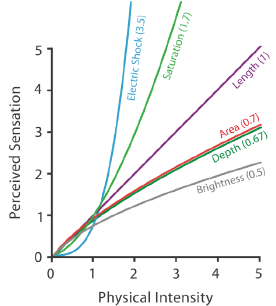
\includegraphics[width=0.3\linewidth]{imgs/lecture3/3.6 law of power.png}
    \caption{The power law of Stevens}
    \label{fig:3.4}
\end{figure}

\subsection{Discriminability}
Match the ranges: the number of different values that one needs to show for the attribute being encoded must not be greater than the number of bins available for the visual channel used to encode it. IF they do not match, one should use a different channel or aggregate the attributes into meaningful bins (highlights the most important one and aggregate all others under the same value, as others).
\subsection{Separability}
Channels may have dependencies and interactions with others, 
\begin{itemize}[noitemsep]
    \item from orthogonal and independent separable channels to the combined integral channels.
    \item Position and hue are completely separable.
    \item Size is not fully separable from color hue.
    \item Horizontal and Vertical size are an integral pair.
\end{itemize}   
\subsection{Pop-out}
Many visual channels provide visual pop-outs, where a distinct item stands out from many others immediately. It has an added value if the time it takes us to spot a different object does not depend on the number of distracting objects.
\begin{figure}[htbp]
    \centering
    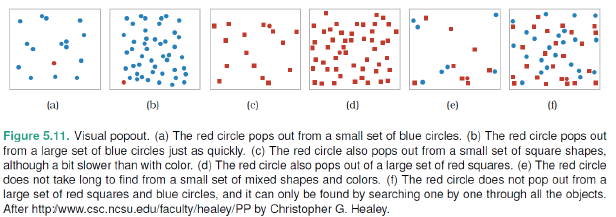
\includegraphics[width=0.5\linewidth]{imgs/lecture3/3.7 pop out.png}
    \caption{Visual pop-out}
    \label{fig:3.7}
\end{figure}
As a general rule, \textit{use pop-out for a single channel at a time}. Most pairs of channels do not support pop-out (except for the shape and color pair). Pop-out is not possible with 2 or more channels
\section{Relative Vs Absolute Judgments}
The human perceptual system is based on relative judgments, not absolute ones. The length difference we can detect is a percentage of the object's length.\par
When two objects are directly next to each other and aligned, we can make a much more precise judgment than when they are not.\par 
Our perception of color and luminance is completely contextual.

\begin{figure}[htbp]
    \centering

    \begin{subfigure}[b]{0.35\linewidth}
        \centering
        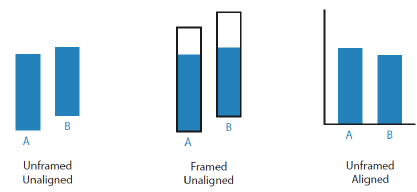
\includegraphics[width=\linewidth]{imgs/lecture3/3.8 relative judgement example 1.png}
        \caption{Are the 2 objects the same height?}
        \label{fig:3.8a}
    \end{subfigure}
    \hfill
    \begin{subfigure}[b]{0.35\linewidth}
        \centering
        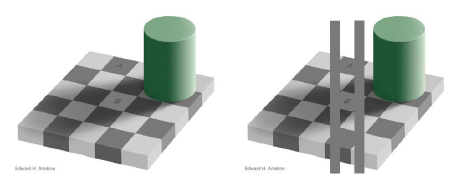
\includegraphics[width=\linewidth]{imgs/lecture3/3.8 relative judgement example 2.png}
        \caption{Are there different shades of gray?}
        \label{fig:3.8b}
    \end{subfigure}
    \hfill

    \caption{Relative judgment examples}
    \label{fig:3.8}
\end{figure}
\chapter{Lecture 4 - Applied Perception}
As we have already seen, information visualization is about transforming data into visual representation so that a human can extract useful information out of it. The effectiveness of a visual representation is not arbitrary; it strongly depends on how brain works. That's why understanding how perception works can help one make informed decisions about visualization designs.

\begin{definition}[Contrast Sensitivity Function]
    Our perception is sensitive to pattern contrast frequency and orientation, also color influences the perception as well. 
\end{definition}

\begin{definition}[Perceptive field in retina]
    The perceptive field of a cell is the visual area over which a cell responds to light. Retinal ganglion cells are organized with circular receptive fields, which are stimulated on-center when excited and stimulated off-center when inhibited.
\end{definition}

\section{Grayscale maps}
The visual effects can result in large errors when reading quantitative information maps displayed using a grayscale map --> use grayscale maps to represent a few values, and not to map or to compare many values.\par
It is useful for highlighting or show boundaries, important items by reducing contrast of unimportant ones; or to adjust background luminance to obtain better readability.

\subsection{Cornsweet illusion}
The lateral inhibition can be considered part of an edge detection process in a scene under viewing. Pseudo-edges can be seen depending on the stimulus.\par
The brain does perceptual interpolation so that regions affected by such edges can appear lighter or darker. This is called \emph{Cornsweet illusion}. 
\begin{figure}[thbp]
    \centering
    
\includegraphics[width=0.4\linewidth]{imgs/lecture4/4.1 cornsweet illusion.png}
    \caption{The Cornsweet effect}
    \label{fig:4.1}
\end{figure}

In the fig~\ref{fig:4.1}, an example of the Cornsweet effect shows the separating line between the shades of gray.

\section{Eye movement}
\begin{itemize}[noitemsep]
    \item \emph{Saccadic} movement: \emph{ballistic} movements of the eyes that change the point of fixation. They can be voluntary or stimulus-elicited
    \item \emph{Smooth-pursuit} movement: \emph{slow tracking} movements of the eyes to keep a moving stimulus on the fovea (a nerve in the eye)
    \item \emph{Vergence} movement: align the fovea of each eye to a target according to its distance
    \item \emph{Vestibulo-ocular} movement: \emph{stabilize} the eyes compensating for head movements
\end{itemize}

\subsection{Saccadic movement and fixations}
The Saccadic eye movements take between 20 to 180 ms. It makes both eyes move in the same direction. This movement may not be a simple linear trajectory.

\begin{definition}[Fixation]
    A fixation is composed of slower and finer movements (microsaccades, tremors, and drift) that help the eye align with the target. A fixation varies between 50 and 600 ms.
\end{definition}

For instance, a typical movement of this kind during reading moves the eyes for 2 degrees, and in general, the movement is between 2 and 5 degrees. If the movement is larger than 20 degrees, the head movement is required.

\section{Pre-attentive process}
Some visual stimuli naturally "pop up" from their surroundings, especially when all the items are of the same characteristics except for one. These "pop-up" features can be: orientation, curvature, shape, size, color, light/dark, enclosure, concavity/convexity, or addition. 

\begin{figure}[htbp]
    \centering

    \begin{subfigure}[b]{0.32\linewidth}
        \centering
        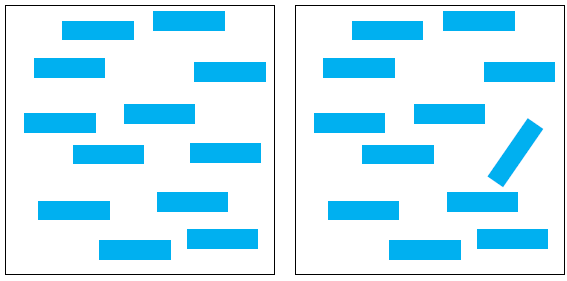
\includegraphics[width=\linewidth]{imgs/lecture4/4.2 preattentive-orientation.png}
        \caption{orientation}
        \label{fig:4.2a}
    \end{subfigure}
    \hfill
    \begin{subfigure}[b]{0.32\linewidth}
        \centering
        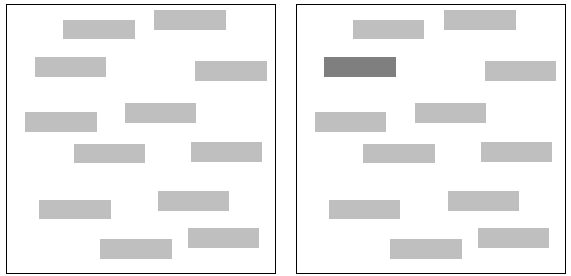
\includegraphics[width=\linewidth]{imgs/lecture4/4.3 preattentive-light dark.png}
        \caption{Light/Dark}
        \label{fig:4.2b}
    \end{subfigure}
    \hfill
    \begin{subfigure}[b]{0.32\linewidth}
        \centering
        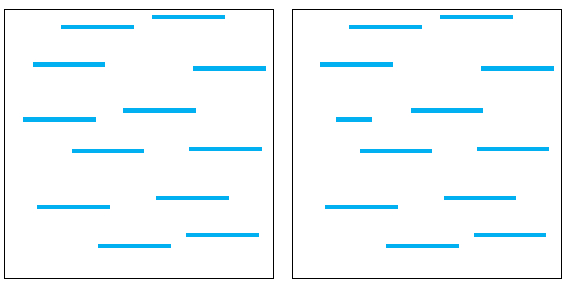
\includegraphics[width=\linewidth]{imgs/lecture4/4.4 preattentive-length.png}
        \caption{Length}
        \label{fig:4.2c}
    \end{subfigure}

    \caption{Features that pop up}
    \label{fig:4.2}
\end{figure}

In the fig~\ref{fig:4.2}, some examples of how some visual features are pre-attentively processed.

\subsection{Asymmetry}
Some pre-attentive processes are not symmetric.
\begin{itemize}[noitemsep]
    \item Adding marks is more efficient than removing marks
    \item Increasing sharpness is more efficient than decreasing sharpness
    \item A big object surrounded by small objects is more efficient than the other way around
\end{itemize}

\begin{figure}[htbp]
    \centering

    \begin{subfigure}[b]{0.32\linewidth}
        \centering
        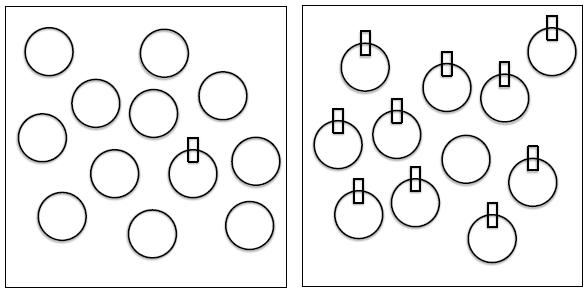
\includegraphics[width=\linewidth]{imgs/lecture4/4.5 asymmetry-marsk.png}
        \caption{Marks}
        \label{fig:4.3a}
    \end{subfigure}
    \hfill
    \begin{subfigure}[b]{0.32\linewidth}
        \centering
        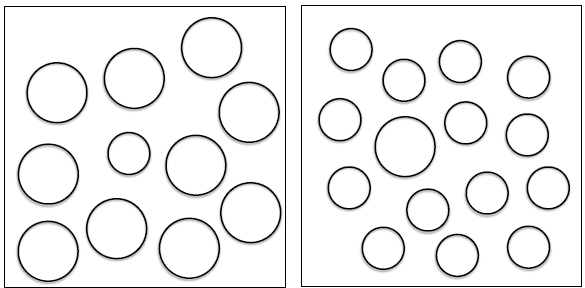
\includegraphics[width=\linewidth]{imgs/lecture4/4.6 asymmetry-size.png}
        \caption{Size}
        \label{fig:4.3b}
    \end{subfigure}
    \hfill
    \begin{subfigure}[b]{0.32\linewidth}
        \centering
        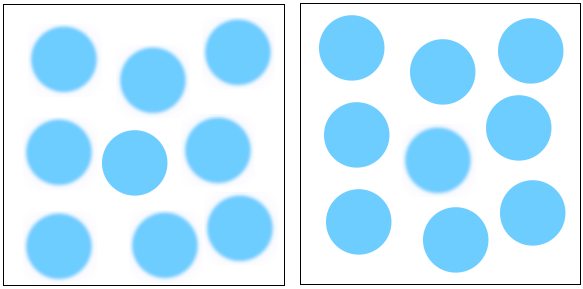
\includegraphics[width=\linewidth]{imgs/lecture4/4.7 asymmetry-sharpness.png}
        \caption{Sharpness}
        \label{fig:4.3c}
    \end{subfigure}

    \caption{Asymmetry of pre-attentive process}
    \label{fig:4.3}
\end{figure}

In the fig~\ref{fig:4.3}, some examples of how some of the asymmetry of the pre-attentive process works. For instance, an object with an additional mark is much more noticeable than an object without a mark.\par

\subsection{Feature combination}
Note that different combinations of pre-attentive visual features may not be pre-attentive.

In the fig~\ref{fig:4.4} shows an example of combining shape and color visual features in an attempt to obtain the "pop up" effect, but the actual result is not as good as we thought.
\begin{figure}[htbp]
    \centering
    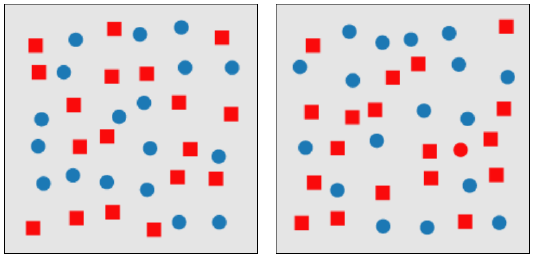
\includegraphics[width=0.4\linewidth]{imgs/lecture4/4.8 preattentive combinations.png}
    \caption{Where is the red circle?}
    \label{fig:4.4}
\end{figure}

\section{Gestalt laws}
It is an attempt to understand pattern perception. It is a powerful ally in visual perception, for example, to show group elements, to show relationships, to make pattern comparisons, in an effective way:
\begin{itemize}[noitemsep]
    \item Proximity: objects close to each other are perceived to form a group
    \item Similarity: similar objects are perceived to form a group
    \item Connectedness: connected objects are perceived as related; most of the time, connecting different objects with a line is a powerful way to express a relationship between the objects.
    \item Continuity: we expect that a line or an edge continues to follow its direction and does not deviate from it
    \item Symmetry: objects arranged symmetrically are perceived as forming a visual whole instead of being perceived as separate entities
    \item Closure: we tend to perceive the complete appearance of an object so that our brain fills the gap in case of missing parts
    \item Common fate: we tend to perceive a group of object that moves in the same direction as a whole
    \item Figure-ground: the perceptual effect regards the formation of a figure from the background
\end{itemize}

\begin{figure}[htbp]
    \centering

    \begin{subfigure}[b]{0.32\linewidth}
        \centering
        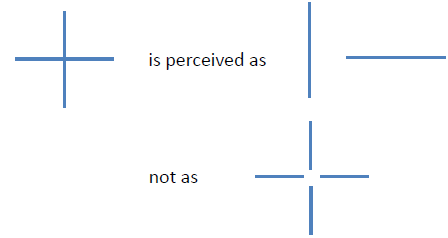
\includegraphics[width=\linewidth]{imgs/lecture4/4.9 connectedness.png}
        \caption{Connectedness}
        \label{fig:4.5a}
    \end{subfigure}
    \hfill
    \begin{subfigure}[b]{0.32\linewidth}
        \centering
        
\includegraphics[width=0.5\linewidth]{imgs/lecture4/4.10 closure.png}
        \caption{Closure}
        \label{fig:4.5b}
    \end{subfigure}
    \hfill
    \begin{subfigure}[b]{0.32\linewidth}
        \centering
        
\includegraphics[width=0.5\linewidth]{imgs/lecture4/4.11 figure ground.png}
        \caption{Figure-ground}
        \label{fig:4.5c}
    \end{subfigure}

    \caption{Gestal laws examples}
    \label{fig:4.5}
\end{figure}
\chapter{Lecture 5 - Applied Perception II}
Color is extremely useful in data visualization to show patterns, for labeling, and for highlighting. However, color is easy to misuse. Think of "color" as an attribute of an object rather than its primary characteristic. 

\section{Basic color perception}
Human have three distinct color receptors on the retina, called the \textit{cones}, which are active at normal light levels. With the support of rods on color perception, we can perceive light or a "shadowy figure" in low luminosity conditions.

\begin{definition}[Trichromacy theory]
    Cones are sensitive to different wavelengths(short, medium, long), hence, they absorb light around the spectrum of \emph{blue, green, and red}. The theory says that we perceive color as a three-channel system. \par
    All color spaces, even if designed to different purposes, as three-dimensional.
\end{definition}

\begin{figure}[htbp]
    \centering
    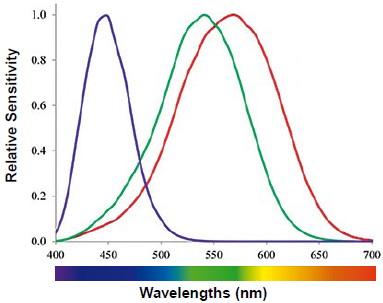
\includegraphics[width=0.3\linewidth]{imgs/lecture5/5.1 thrichromacy theory.png}
    \caption{Thrichromacy theory}
    \label{fig:5.1}
\end{figure}

\subsection{Color measurement and specification}
Since only three different receptors are involved in color vision, it is possible to match a patch of color light using a mixture of three color lights, called \emph{primaries}. The color experiment consists in using a transformation to create the same color on different output devices. \par
In fig~\ref{fig:5.2a} we show the experiment setup and results, the goal of the experiment is represented in "making screen", adjust the colors so that the two halves of the circle show the same color.\par
In fig~\ref{fig:5.2b} we show the experiment result on how sensitive our eyes perceive the primaries, the so-called \textbf{RGB color space}, created by the CIE - International Commission of Color.

\begin{figure}[htbp]
    \centering

    \begin{subfigure}[b]{0.4\linewidth}
        \centering
        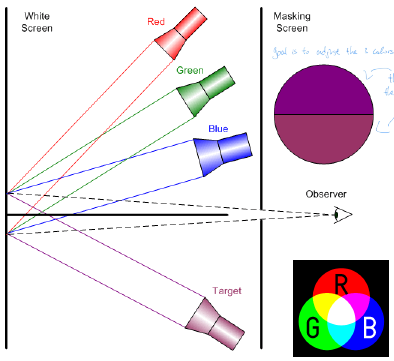
\includegraphics[width=\linewidth]{imgs/lecture5/5.2 color experiment.png}
        \caption{Experiment setup}
        \label{fig:5.2a}
    \end{subfigure}
    \hfill
    \begin{subfigure}[b]{0.4\linewidth}
        \centering
        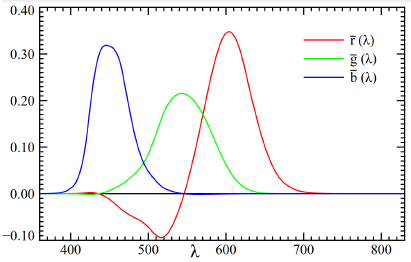
\includegraphics[width=\linewidth]{imgs/lecture5/5.3 color results.png}
        \caption{Experiment results as functions}
        \label{fig:5.2b}
    \end{subfigure}

    \caption{Color measurement experiment}
    \label{fig:5.2}
\end{figure}

The RGB color matching function can also be represented as a \textit{function of X, Y, and Z}, where:
\begin{itemize}[noitemsep]
    \item Y corresponds to the perceived luminance in well-lit condition
    \item Z is close to the short cone response
    \item X is a mix such that the values become non-negative
\end{itemize}
And for a fixed value of Y, the plane XZ contains all the possible chromaticities at that luminance.

\begin{figure}[htbp]
    \centering

    \begin{subfigure}[b]{0.4\linewidth}
        \centering
        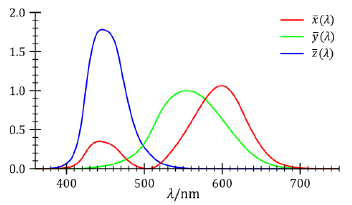
\includegraphics[width=\linewidth]{imgs/lecture5/5.4 xyz color matching.png}
        \caption{Color matching function as XYZ}
        \label{fig:5.3a}
    \end{subfigure}
    \hfill
    \begin{subfigure}[b]{0.4\linewidth}
        \centering
        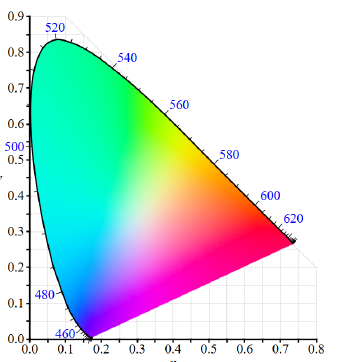
\includegraphics[width=0.5\linewidth]{imgs/lecture5/5.5 chromaticity diagram.png}
        \caption{Chromaticity diagram}
        \label{fig:5.3b}
    \end{subfigure}

    \caption{XYZ color space}
    \label{fig:5.3}
\end{figure}

\begin{definition}[Gamut]
    Gamut is the set of color spaces that a device, such as a printer or a monitor can reproduce. Most of the time, it is a subspace of the chromaticity diagram
\end{definition}

\subsection{Opponent process theory}
The theory was proposed by Hering, a German psychologist, and later supported by experiments. Hering proposed that cones combine their stimulus, forming three pairs of colors that compete to form the final one. These pairs, called \emph{opponent pairs} are \emph{black-white, red-green, and yellow-blue}.\par
This theory suggests that the visual system interprets color by processing signals from three types of cone cells in an antagonistic manner, meaning that the activation of one color inhibits the perception of its opposite.\par
One interesting implication is the \emph{afterimages}. For example, if you stare at a bright color (like red) for a long period of time and then look at a white-colored surface, you may see a cyan afterimage. This happens because the red receptors become fatigued, leading to the perception of their complementary color. \par 
It also suggests the extremes of the opponent channels, which are fundamental to our understanding of color perception. These unique hues are \emph{red, green, blue} which cannot be created by mixing other colors.

\begin{figure}[htbp]
    \centering
    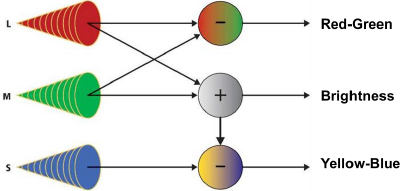
\includegraphics[width=0.4\linewidth]{imgs/lecture5/5.6 opponent process theory.png}
    \caption{Opponent process theory}
    \label{fig:5.4}
\end{figure}

In fig~\ref{fig:5.5} shows an example of this theory in practice. When looking at this picture for at least 30 seconds, and focus at the little white dot in the middle. Then switch to a white colored surface, and what we see on the white background is the flag of the USA. This is because when you stare at these colors, you are exciting the same source of these colors, and when you switch to the white background, since these sensors have been excited for too long, they inhibit those colors as the only colors.

\begin{figure}[htbp]
    \centering
    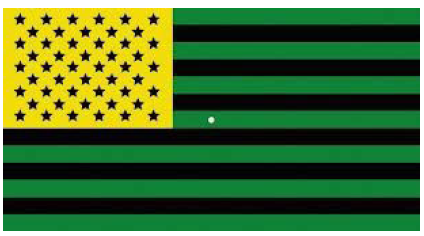
\includegraphics[width=0.3\linewidth]{imgs/lecture5/5.7 opponent process theory-example.png}
    \caption{Opponent process theory, an example}
    \label{fig:5.5}
\end{figure}

\section{Color spaces}
\textbf{Saturation} means how pure the color is, intended as its brightness.

\begin{figure}[htbp]
    \centering
    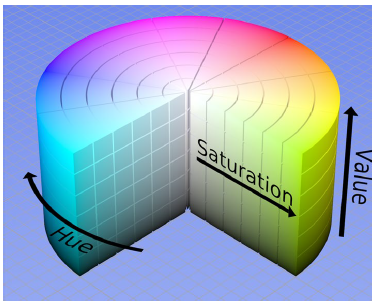
\includegraphics[width=0.3\linewidth]{imgs/lecture5/5.8 hue saturation values.png}
    \caption{Hue Saturation Value}
    \label{fig:5.6}
\end{figure}

Color specification can be represented as in fig~\ref{fig:5.6}, which is a more natural representation than with RGB. But, they are not perceptually uniform spaces (calculated Euclidean distance in the color space does not correspond to perceptual distances).\par
Having a color space in which equal perceptual distances are useful to specify color tolerances, color codes, pseudo-coloring using sequences of colors to represent data values, possibly with perceptually equal steps.\par

The Euclidean distance is meaningful from a perceptual point of view for the color space. It is defined in eq~\ref{eq:5.1}.
\begin{equation}
    \Delta E_{ab}^{*} = \sqrt{(L_2^{*} - L_1^{*})^2 + (a_2^{*} - a_1^{*})^2 + (b_2^{*} - b_1^{*})^2}
    \label{eq:5.1}
\end{equation}

If the result \(\Delta E\) < 1, colors are not perceptible; for 1 < \(\Delta E\) < 2, close observation needed to perceive the difference; for 2 < \(\Delta E\) < 10, the colors are similar but different. It is important to know that \(\Delta E\) is not perceptually uniform as originally intended and therefore suspended by specifications.\par
Although uniform color spaces only provide a rough first approximation of how color differences will be perceived, an important influencing factor is size: we are much more sensitive to differences between large patches. \par
\textit{Tips}: Use saturated colors when coding small symbols or thin lines, and less saturated colors for large areas, as showed in fig~\ref{fig:5.7}.

\begin{figure}[htbp]
    \centering
    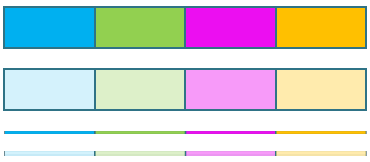
\includegraphics[width=0.3\linewidth]{imgs/lecture5/5.9 color differences.png}
    \caption{Color differences and use of saturation}
    \label{fig:5.7}
\end{figure}

\section{Color and Visualization}
The red-green and yellow-blue chromatic channels presented from the opponent process theory are each capable of carrying only about 1/3 of the amount of detail carried by the black-white channel.\par
Purely chromatic differences are not enough to display fine details, ensuring adequate luminance contrast with the background, and also colors with different chromaticity (saturation) can be used to improve readability.

\begin{figure}[htbp]
    \centering

    \begin{subfigure}[b]{0.4\linewidth}
        \centering
        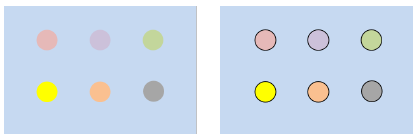
\includegraphics[width=\linewidth]{imgs/lecture5/5.10 visualization and luminance.png}
        \caption{Contrast boundary to improve readability}
        \label{fig:5.8a}
    \end{subfigure}
    \hfill
    \begin{subfigure}[b]{0.4\linewidth}
        \centering
        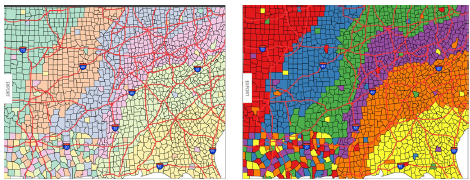
\includegraphics[width=\linewidth]{imgs/lecture5/5.11 visualization and saturation.png}
        \caption{Less saturated colors for large patches and saturated colors for finer details}
        \label{fig:5.8b}
    \end{subfigure}

    \caption{Visualization and color properties}
    \label{fig:5.8}
\end{figure}

In 1986, Post and Greene carried out an experiment on the naming of colors; among 210 different colors, only 8, plus white, were consistently named. This result suggests that only a few colors can be used as categorical labels. Nowadays, the 12 recommended colors shown in fig~\ref{fig:5.9} are widely agreed-upon category names with reasonably far apart in color space. These colors are: red, yellow, black, pink, gray, brown, green, blue, white, cyan, orange, purple.

\begin{figure}[htbp]
    \centering
    
\includegraphics[width=0.3\linewidth]{imgs/lecture5/5.12 color labels.png}
    \caption{Color labels}
    \label{fig:5.9}
\end{figure}

\subsubsection{Color and Semantics}
There are no universal conventions on associating a color with some semantics, but they are widely used. For instance, red for hot/bad/danger, blue for cold, green for life/go, etc. The semantic association with gray is that of belonging to an unspecified category, which can be used for highlighting more important information using different colors. 

\subsubsection{Color ramps}
Color ramps are a predefined set of colors used to present a theme (green-yellow hue of colors represents summer, red-orange-yellow hue of colors represents autumn ...).\par
There are some guidelines in using color ramps, for instance, avoid color ramps problematic for color-blind individuals; use a spectrum-based color ramp when its use is deeply embedded in the user culture; to reveal fine details, use a pseudo-color sequence that varies in luminance, not only in chromaticity. 
\chapter{Lecture 6 - Tables}
\begin{definition}[Key and Value]
    A \emph{key} is an independent attribute that can be used as a unique index to look up items in a table, while a \emph{value} is a dependent attribute. \par
    When deciding on the visualization, one should know the number of keys and the number of values in the table, so that different types of tables can be more suitable.
\end{definition}
\section{Scatterplot}
Scatterplot encodes two quantitative attributes (values) using vertical and horizontal spatial position channels, and the mark type is point. It is effective for providing overviews and characterizing distributions, specifically for finding outliers and extreme values. It can also be used to judge the correlation between 2 attributes.\par
\subsubsection{Correlation}
With Visual encoding, the task corresponds to the easy perceptual judgment of noticing whether the points form a line along the diagonal. The stronger the correlation, the closer the points fall along a perfect diagonal line; positive correlation is an upward slope, and negative correlation is a downward slope. In addition, a regression line is often superimposed on the raw scatterplot to show the best fit between attributes. One can even use a transformation to derive a clearer relationship between attributes. It is suited for up to hundreds of points (items) for the scalability issue.

\begin{figure}[htbp]
    \centering
    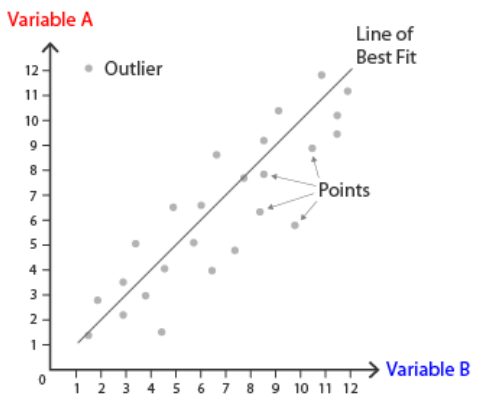
\includegraphics[width=0.35\linewidth]{imgs/lecture6/6.1 scatterplot correlation.png}
    \caption{Scatterplot for feature correlation}
    \label{fig:6.1}
\end{figure}

\subsubsection{Recap: Scatterplot}
\begin{tabularx}{0.8\textwidth} { 
  | >{\raggedright\arraybackslash}l 
  | >{\raggedright\arraybackslash}X | }
    \hline
    Data (What) & Table with 2 quantitative value attributes \\
    \hline
    Encode (How) & Express values with horizontal and vertical spatial position and point marks \\
    \hline
    Task (Why) & Find trends, outliers, distribution, correlation; locate clusters\\
    \hline
    Scale &  hundreds of items\\
    \hline
\end{tabularx}

\section{Bar chart}
A bar chart uses a line mark and usually encodes a categorical or ordinal key attribute using position along the horizontal axis as a channel and a quantitative value attribute with position along the vertical axis. Each bar is in a separate region of space, and there is one for each level of the categorical attribute.\par
It is useful to visualize how a measured quantity is distributed across categories, and also for looking up individual values. Bars are all aligned within a common frame, so that the highest-accuracy aligned-position channel is used.\par
Bars can be ordered alphabetically by the categories, which makes look-up by name easy, but often hinders the meaningful patterns in the dataset. Another ordering is by the values of the quantitative attribute that is encoded by the bar heights; this data-driven ordering makes it easier to see dataset trends. \par
The scalability is a big issue here; to accommodate bars, sufficiently large white space should be allocated so that each bar line mark is distinguishable. \textit{Less is more...}

\subsubsection{Percentage stacked bar chart}
Unlike a simple stacked bar chart, which uses the absolute values. Percentage bar chart uses the normalized values so that the sum of segments in a single bar is 100\%. This can be used to better show the relative difference between quantities in the different groups.

\subsubsection{Recap: Bar charts}
\begin{tabularx}{0.8\textwidth} { 
  | >{\raggedright\arraybackslash}l 
  | >{\raggedright\arraybackslash}X | }
    \hline
    Data (What) & Table with one quantitative value attribute and one categorical key attribute \\
    \hline
    Encode (How) & Line marks, express value attribute with aligned vertical position, separate key attribute with horizontal position \\
    \hline
    Task (Why) & Lookup and compare values\\
    \hline
    Scale &  up to hundreds of levels of key attributes\\
    \hline
\end{tabularx}

\section{Histogram}
A histogram visualizes the distribution of values of a quantitative attribute. It uses the same marks and channels as bar charts, but a histogram usually shows derived or aggregated data; there is no space between bars; it shows the continuous distribution of the data, and thus makes no sense to order bars.

\begin{figure}
    \centering
    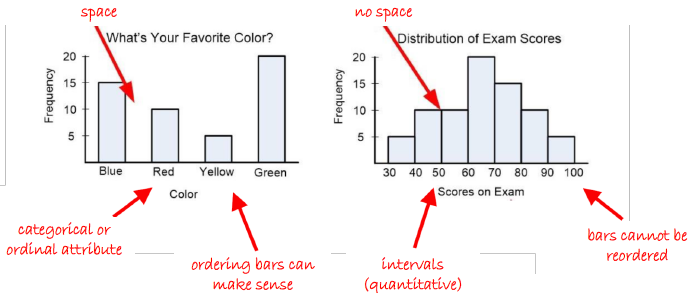
\includegraphics[width=0.5\linewidth]{imgs/lecture6/6.2 bar chart and histogram.png}
    \caption{Difference between a bar chart and a histogram}
    \label{fig:6.2}
\end{figure}

\subsubsection{Recap: Histogram}
\begin{tabularx}{0.8\textwidth} { 
  | >{\raggedright\arraybackslash}l 
  | >{\raggedright\arraybackslash}X | }
    \hline
    Data (What) & Table with one quantitative value attribute \\
    \hline
    Derived (What) & Derived table is the one where one derived ordered key attribute (bin) and one derived quantitative value attribute (item count per bin) \\
    \hline
    Encode (How) & Rectilinear layout, line mark with aligned position to express derived value attribute. Position is judged by key attribute \\
    \hline

\end{tabularx}

\section{Line chart}
A line chart visualizes an ordered key attribute using horizontal position as a channel and a quantitative value attribute using vertical position as a channel. \par
The marks are points and line segments connecting consecutive point pairs. Segments are connection marks to emphasize the ordering of the items along the key ais by explicitly showing the relationship between one item and the next. Thus, they have a stronger implication of trend relationships, making them suitable for the task of spotting trends. Its popular applications include finance, climate studies, public policies ...

\subsubsection{Area Chart} It is a variation of line charts with the area below the line filled in.

\subsubsection{Recap: Line charts}
\begin{tabularx}{0.8\textwidth} { 
  | >{\raggedright\arraybackslash}l 
  | >{\raggedright\arraybackslash}X | }
    \hline
    Data (What) & Table with one quantitative value attribute and one ordered key attribute \\
    \hline
    Encode (How) & Dot chart with connection marks between dots \\
    \hline
    Task (Why) & Show trend\\
    \hline
    Scale &  up to hundreds of levels of key attributes\\
    \hline
\end{tabularx}

\section{Multiple attributes}
\subsection{Bubble Chart}
It is a variation on a scatterplot, accommodated to represent additional attributes, where circle areas and colors can represent additional attributes. One could add even more channels and attributes, but it would also make information decoding much harder. Too many bubbles can make the chart hard to read; therefore, bubble charts have a limited data size capacity. However, this can be solved through interactivity, by, for example, a filter for categories, clicking over a bubble to display hidden information, and so on.

\begin{figure}[htbp]
    \centering
    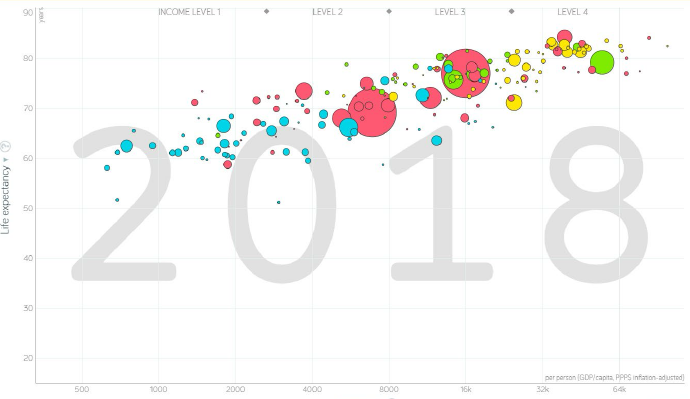
\includegraphics[width=0.3\linewidth]{imgs/lecture6/6.3 bubble chart.png}
    \caption{Bubble chart}
    \label{fig:6.3}
\end{figure}

\subsection{Stacked Bar chart}
It is a more complex glyph for each bar, with multiple sub-bars stacked vertically. It has two key attributes that can have as many composite bars as the number of values for the first key attribute and as many sub-components within each bar as the values for the other key attribute. Both the length of the composite bar and the length of each sub-component encode values, resulting in a multidimensional table.\par
Composite glyphs are arranged horizontally according to the primary key; the secondary key is used to construct the vertical structure of the glyph, and color is often used alongside length coding.

\begin{figure}[htbp]
    \centering
    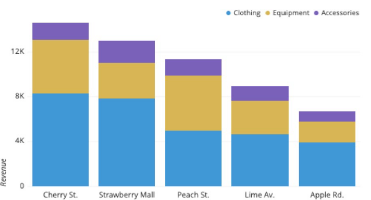
\includegraphics[width=0.4\linewidth]{imgs/lecture6/6.4 stacked bar chart.png}
    \caption{Stacked bar chart}
    \label{fig:6.4}
\end{figure}

In fig~\ref{fig:6.4} shows an example of a stacked bar chart: 
\begin{itemize}[noitemsep]
    \item the full bar height (representing the first key attribute) shows the value for the combination of all items in the stack; 
    \item the height of the full combined bar and the lowest sub-component is easy to read and to compare against each other because they have an aligned starting point
    \item each sub-component is represented with a different color, which represents the second key attribute, it has as many values as the number of sub-components (also color, in this case)
    \item The ordering of stacking is significant, as it determines the patterns that are most easily visible
\end{itemize}

\subsubsection{Recap: Stacked Bar charts}
\begin{tabularx}{0.8\textwidth} { 
  | >{\raggedright\arraybackslash}l 
  | >{\raggedright\arraybackslash}X | }
    \hline
    Data (What) & Multidimensional table with one quantitative value attribute and two categorical key attributes \\
    \hline
    Encode (How) & Bar glyph with length-coded sub-components of value attribute for each category of secondary attribute. Separate bars by category of primary key attribute \\
    \hline
    Task (Why) & Part-to-whole relationship, lookup values, find trends\\
    \hline
    Scale &  up to hundreds of levels for the main axis key attributes. Several levels for the secondary (stacked glyph axis) key attribute\\
    \hline
\end{tabularx}

\subsubsection{Normalized Stacked Bar chart}
It is a variant of stacked bar chart in which the quantitative attribute is normalized, showing proportion instead of absolute values

\subsubsection{Grouped Bar chart}
It is another representation of a stacked bar chart, with two key attributes. The same bar chart is repeated multiple times for the number of categories in the second attribute. It is an excellent tool for the comparison of individual values

\begin{figure}[htbp]
    \centering

    \begin{subfigure}[b]{0.4\linewidth}
        \centering
        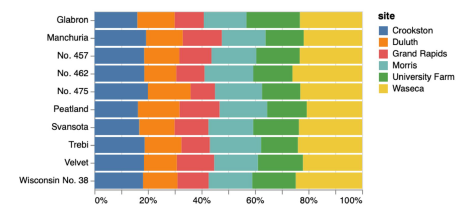
\includegraphics[width=\linewidth]{imgs/lecture6/6.5 normalized stacked bar chart.png}
        \caption{Normalized Stacked Bar chart}
        \label{fig:6.5a}
    \end{subfigure}
    \hfill
    \begin{subfigure}[b]{0.4\linewidth}
        \centering
        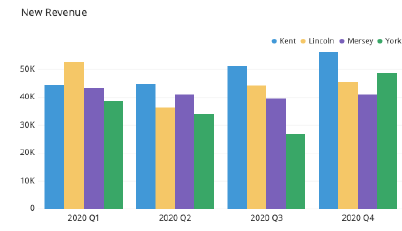
\includegraphics[width=\linewidth]{imgs/lecture6/6.6 grouped bar chart.png}
        \caption{Grouped Bar chart}
        \label{fig:6.5b}
    \end{subfigure}

    \caption{Bar chart variations}
    \label{fig:6.5}
\end{figure}

\subsection{Line chart variations}
\subsubsection{Stacked Line chart}
A variation of a line chart in which values across categories are stacked one on top of each other. It has a big noticeable limitation: it is not good for reading and comparing individual values over time, since the values are stacked, and the shape of lines is affected by the shape of lines below it. This can be somehow mediated through a filter interaction. It can be meaningless for data that shouldn't be summed, like temperature.

\subsubsection{Line chart Series}
It is a collection of lines in the same chart, easy to use, and has high readability, but to be careful to not to overfill the chart with lines.

\subsubsection{Small multiples}
An alternative way to show multiple attributes that hold for all types of charts by creating multiple replicas of the same graph, with each graph in its own chart. It is sometimes more effective than a single plot including too much data.

\subsubsection{Flow maps}
Depict the movement of entities in space and time by placing stroked lines on top of maps. A flow map encode a large amount of multivariate information (thickness, color, etc. can encode additional information)

\begin{figure}[htbp]
    \centering

    \begin{subfigure}[b]{0.32\linewidth}
        \centering
        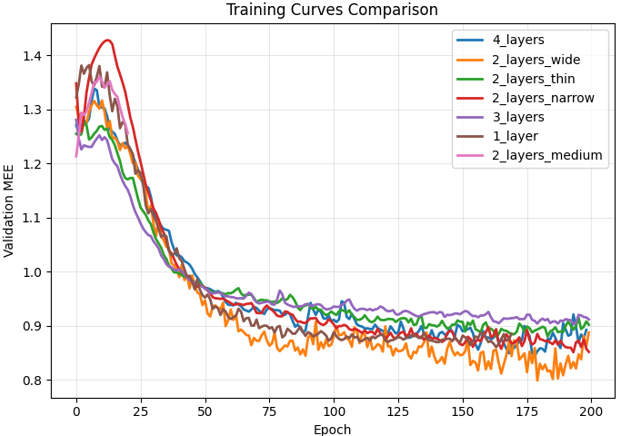
\includegraphics[width=\linewidth]{imgs/lecture6/6.7 line chart series.png}
        \caption{Line chart series}
        \label{fig:6.6a}
    \end{subfigure}
    \hfill
    \begin{subfigure}[b]{0.32\linewidth}
        \centering
        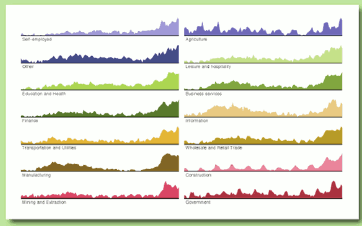
\includegraphics[width=\linewidth]{imgs/lecture6/6.8 small multiples.png}
        \caption{Small multiples}
        \label{fig:6.6b}
    \end{subfigure}
    \hfill
    \begin{subfigure}[b]{0.32\linewidth}
        \centering
        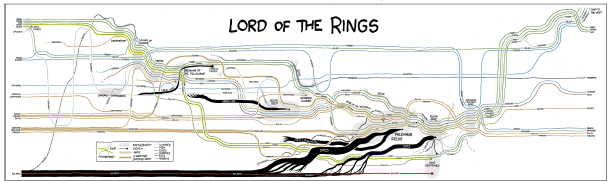
\includegraphics[width=\linewidth]{imgs/lecture6/6.9 flow map.png}
        \caption{Flow map}
        \label{fig:6.6c}
    \end{subfigure}

    \caption{Line chart variations}
    \label{fig:6.6}
\end{figure}

\subsection{Heatmap}
A heatmap is a 2-dimensional matrix alignment to arrange two key attributes and one value attribute. One key is distributed along the rows and the other along the columns; each rectangular cell in the matrix is occupied by an area mark encoding a single quantitative value attribute with color. \par
The use of a heatmap allows us to visually encoding quantitative data with color using small area marks, making it very compact. It is good for overviews with high information density and is highly scalable. Keys can also be ordered to identify patterns, even if it is a categorical attribute (can be ordered according to color). \par
But, its use discriminates a large number of distinct values; only a small number of different levels of the quantitative attribute can be distinguishable, because of the limits of color perception in small, non-contiguous regions.

\begin{figure}[htbp]
    \centering
    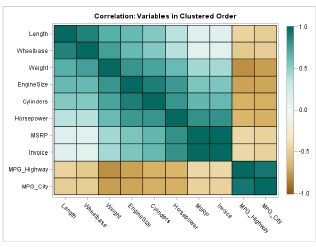
\includegraphics[width=0.5\linewidth]{imgs/lecture6/6.15 heatmap.png}
    \caption{Heatmap}
    \label{fig:6.7}
\end{figure}

\subsubsection{Recap: Heatmap}
\begin{tabularx}{0.8\textwidth} { 
  | >{\raggedright\arraybackslash}l 
  | >{\raggedright\arraybackslash}X | }
    \hline
    Data (What) & Table with one quantitative value attribute and two categorical key attributes \\
    \hline
    Encode (How) & A 2D matrix alignment of area marks, diverging color map \\
    \hline
    Task (Why) & Find clusters, outliers, summarize\\
    \hline
    Scale &  Can have up to one million items; hundreds of levels of categorical attributes; tens of levels of quantitative attributes\\
    \hline
\end{tabularx}

\section{Other visualization tables}
\subsubsection{Wordcloud}
It is a representation of how frequently words appear in a given body of text through the size of the word. It can have various variations in arrangement and color. Mainly used for aesthetic reasons.
\subsubsection{Calligrams}
It is an image created by arranging the texts to form a thematically related image
\subsubsection{Multidimensional icons}
The graph that encode properties of an object in a simple iconic representation. 
\subsubsection{Petals as glyph}
The graph visualize a life index, it maps several variables related to material living conditions and quality of life into petals of different size, to compare well-being across countries. 
\subsubsection{Chernoff faces}
It is introduces based on the assumption that human are good at recognizing faces. Variables are mapped to facial features (width/curvature of mouth, vertical size of face, size/slant/separation of eyes, size of eyebrows...). It needs a legend. \textit{It is not a pre-attentive process...?}

\begin{figure}[htbp]
    \centering
    
    % First row (3 images)
    \begin{subfigure}{0.32\textwidth}
        \centering
        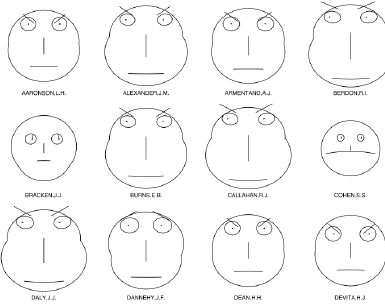
\includegraphics[width=\linewidth]{imgs/lecture6/6.14 chernoff faces.png}
        \caption{Chernoff faces}
        \label{fig:6.8a}
    \end{subfigure}
    \hfill
    \begin{subfigure}{0.3\textwidth}
        \centering
        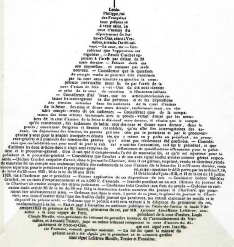
\includegraphics[width=\linewidth]{imgs/lecture6/6.11 calligram.png}
        \caption{Calligram}
        \label{fig:6.8b}
    \end{subfigure}
    \hfill
    \begin{subfigure}{0.3\textwidth}
        \centering
        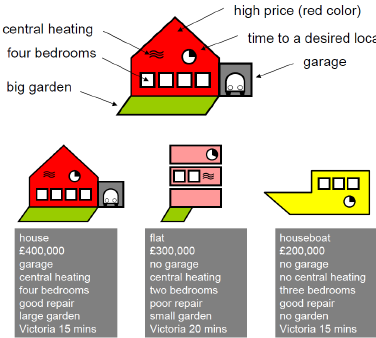
\includegraphics[width=\linewidth]{imgs/lecture6/6.12 multidimentional icons.png}
        \caption{Multidimensional icons}
        \label{fig:6.8c}
    \end{subfigure}

    \vspace{0.5cm}

    % Second row (2 images)
    \begin{subfigure}{0.45\textwidth}
        \centering
        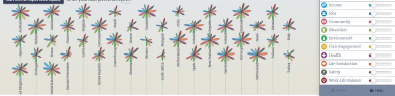
\includegraphics[width=\linewidth]{imgs/lecture6/6.13 petals as glyph.png}
        \caption{Petal as glyph}
        \label{fig:6.8d}
    \end{subfigure}
    \hfill
    \begin{subfigure}{0.45\textwidth}
        \centering
        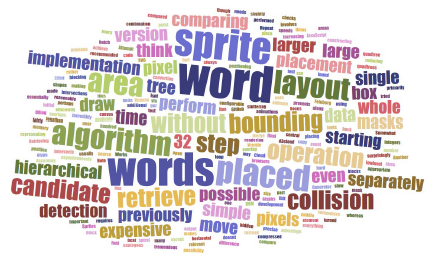
\includegraphics[width=\linewidth]{imgs/lecture6/6.10 wordcloud.png}
        \caption{Wordcloud}
        \label{fig:6.8e}
    \end{subfigure}

    \caption{Other visualization tables}
    \label{fig:6.8}
\end{figure}
\chapter{Lecture 7 - Charts}
Spatial axes are an important ingredient in visualization. One should always label the axes and set the standard unit of distance between two points in the chart. This layout can be:
\begin{itemize}[noitemsep]
    \item rectilinear: items distributed along two perpendicular axes, with values ranging from a minimum to a maximum. (like in most of the tables mentioned in Chapter 6)
    \item parallel: axes placed parallel to each other (in the case of a slope chart)
    \item radial: items distributed around a circle, using the angle channel (like in a pie chart)
\end{itemize}

\subsubsection{Radial layout}
Items in a radial layout are distributed around a circle, using the angle channel. The most natural coordinate system in radial layout is polar coordinates, where one dimension is measured as an angle from a starting line, and the other dimension is measured as a distance from a center point. Compared to a rectilinear spatial position channel, the angle channel is less accurately perceived.

\section{Radial bar chart}
The radial bar chart is similar to a bar chart, using the same line marks to encode a quantitative attribute with the length channel, the only difference being the radial vs rectilinear orientation of the axes. This chart can be messy to the eye; it is usually a good idea to re-order the bars to that the comparison from the highest to the smallest values can be perceived. This chart can be revisited to encode multiple attributes. 

\begin{figure}[htbp]
    \centering

    \begin{subfigure}[b]{0.4\linewidth}
        \centering
        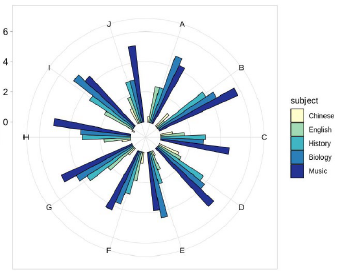
\includegraphics[width=0.5\linewidth]{imgs/lecture7/7.1 radial bar chart.png}
        \caption{encoding multiple attributes}
        \label{fig:7.1a}
    \end{subfigure}
    \hfill
    \begin{subfigure}[b]{0.4\linewidth}
        \centering
        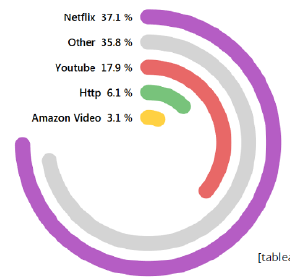
\includegraphics[width=0.5\linewidth]{imgs/lecture7/7.2 radial bar chart.png}
        \caption{different forms of radial bar chart}
        \label{fig:7.2b}
    \end{subfigure}

    \caption{Different use of radial bar chart}
    \label{fig:7.1}
\end{figure}

\subsubsection{Recap: Radial bar chart}
\begin{tabularx}{0.8\textwidth} { 
  | >{\raggedright\arraybackslash}l 
  | >{\raggedright\arraybackslash}X | }
    \hline
    Data (What) & Table with one quantitative value attribute and one categorical key attribute \\
    \hline
    Encode (How) & Length coding of line marks, radial layout \\
    \hline
\end{tabularx}

\section{Pie chart}
The pie chart is the most commonly used radial graphic; it uses 2D area marks and the angle (arc length) channel. It is used to show percentages and proportions among categories by dividing a circle into proportional segments, with each angle/arc length representing the value/proportion for each category, and the full circle represents the sum of all data, i.e., 100\%. \par
Despite the popularity, pie charts are clearly problematic when considered according to the visual channel properties. While it is useful for giving a quick idea and to compare one slice against the total, it is not good for an accurate comparison: angle judgments on area marks are less accurate than length judgments on line marks; the wedges vary in width along the radial axis, from narrow near the center to wide near the end, making the area judgments difficult. In addition, scalability is an issue; it can shows up to tens of categories, simply because as the number of categories increases, the size of each segment decreases, not to mention the size of the legend would also become proportionally large. \par
The most useful property of pie charts is that they show the relative contribution of parts to a whole; however, this property is unique to pie charts. A single bar in a normalized stacked bar chart would do the same job with a more accurate channel of length.\par
A pie chart is also one of the most commonly \textit{misused} visualization:
\begin{itemize}[noitemsep]
    \item sum of the percentage of all slices differ from 100\%
    \item redundant representations of data (sometimes people would put a number, a percentage of the slice to the whole, together with the slice)
    \item unnecessary and unjustified channel, like 3D (applies to all types to visualization)
    \item incomplete pie chart showing only some slices, \textit{but}, depending on the context, it can be useful for emphasizing the portion on the given topic, thus, showing comparison between different subjects.
\end{itemize}

\begin{figure}[htbp]
    \centering
    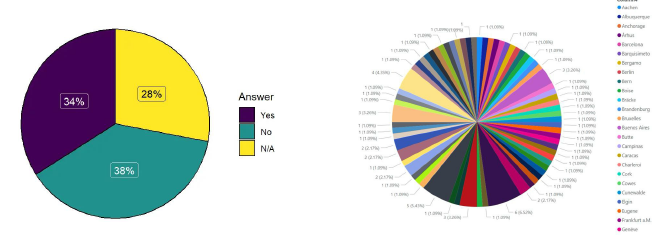
\includegraphics[width=0.5\linewidth]{imgs/lecture7/7.3 pie chart misuse.png}
    \caption{Pie chart misuses}
    \label{fig:7.2}
\end{figure}

\subsubsection{Donut chart}
It is a variant of a pie chart with the center area cut out, making the focus on arc length rather than on area. It is more efficient on space occupancy while providing more space for labels.

\subsubsection{Polar area chart}
Another variation of a pie chart that varies the length of the wedge, rather than varying angles. 

\subsubsection{Radar chart}
Also called a spider chart or star chart, where items are displayed along circles, it is useful for periodic data. This chart can easily compare properties of a class of objects or a category, but not as much in understanding the trade-off between variables. One should be careful when using it for many variables or many data points.

\subsubsection{Sunburst chart}
It has a radial layout but can be used to visualize hierarchies. A sunburst chart visualizes hierarchies (a tree structure) with concentric circles where each ring represents a level in the hierarchy, moving outwards. \par
It used multiple channels, such as distances from the center representing levels in the hierarchy, the angle representing connections among items (nodes), and color can also give additional information about the items. Note that each ring does not have to be complete, as a tree does not have to be perfectly balanced.

\begin{figure}[htbp]
    \centering
    
    % First row (3 images)
    \begin{subfigure}{0.45\textwidth}
        \centering
        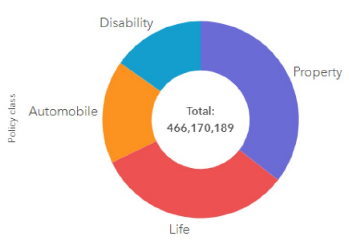
\includegraphics[width=0.7\linewidth]{imgs/lecture7/7.4 donut chart.png}
        \caption{Donut chart}
        \label{fig:7.3a}
    \end{subfigure}
    \hfill
    \begin{subfigure}{0.45\textwidth}
        \centering
        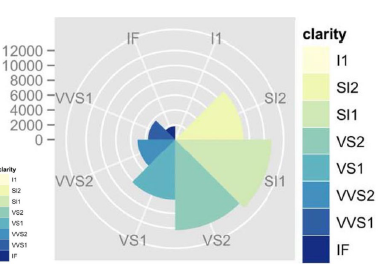
\includegraphics[width=0.7\linewidth]{imgs/lecture7/7.5 polar area chart.png}
        \caption{Polar area chart}
        \label{fig:7.3b}
    \end{subfigure}

    \vspace{0.5cm}

    % Second row (2 images)
    \begin{subfigure}{0.45\textwidth}
        \centering
        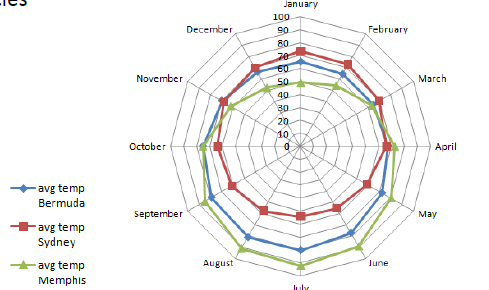
\includegraphics[width=0.7\linewidth]{imgs/lecture7/7.6 spider chart.png}
        \caption{Radar chart (or spider chart)}
        \label{fig:7.3c}
    \end{subfigure}
    \hfill
    \begin{subfigure}{0.45\textwidth}
        \centering
        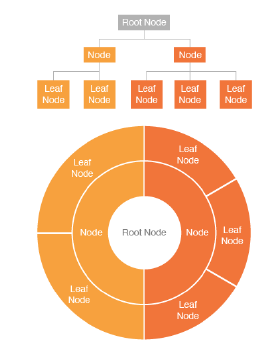
\includegraphics[width=0.7\linewidth]{imgs/lecture7/7.7 sunburst chart.png}
        \caption{Sunburst chart}
        \label{fig:7.3d}
    \end{subfigure}

    \caption{Variations of a pie chart}
    \label{fig:7.3}
\end{figure}

\section{Treemap}
A treemap is an alternative way to visualize hierarchies, by displaying quantities via area size. Each rectangle represents a category, with nested subcategory rectangles. Child nodes are contained in the area region representing the parent node. When a quantity is assigned to a category, its area size is displayed in proportion to that quantity and to the other quantities within the same parent category in a part-to-whole relationship.\par
The treemap is very compact and space-efficient, but it is not as good as a sunburst chart in showing the levels in the hierarchy, because only leaf attributes are displayed. In general, it is a good option for showing the overall structure and providing an estimated comparison via area sizes.

\subsubsection{Bubble hierarchy}
As with a treemap, it uses containment to represent hierarchies and area to visualize quantities, but with bubbles-shaped containers rather than rectangles. 

\begin{figure}[htbp]
    \centering
    
    \begin{subfigure}{0.45\textwidth}
        \centering
        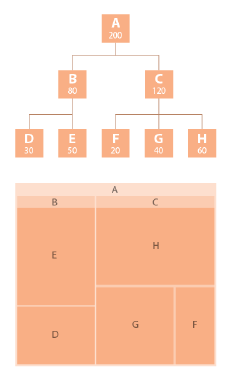
\includegraphics[width=0.6\linewidth]{imgs/lecture7/7.8 treemap.png}
        \caption{Treemap}
        \label{fig:7.4a}
    \end{subfigure}
    \hfill
    \begin{subfigure}{0.45\textwidth}
        \centering
        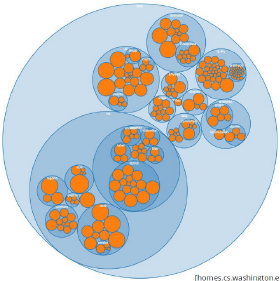
\includegraphics[width=0.5\linewidth]{imgs/lecture7/7.9 bubble hierarchy.png}
        \caption{Bubble hierarchy}
        \label{fig:7.4b}
    \end{subfigure}

    \caption{Treemap and Bubble hierarchy variant}
    \label{fig:7.4}
\end{figure}

\subsection{Different representations of a tree dataset}
\begin{figure}[htbp]
    \centering
    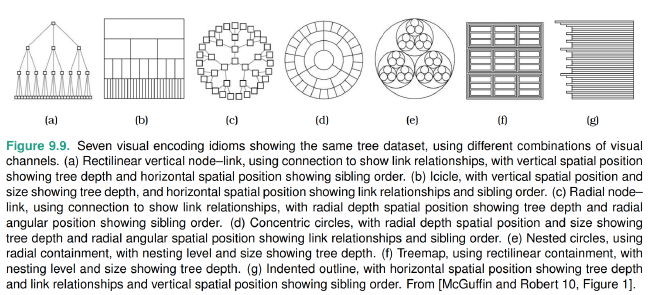
\includegraphics[width=0.88\linewidth]{imgs/lecture7/7.10 visualizing a tree.png}
    \caption{Visualizing a tree dataset}
    \label{fig:7.5}
\end{figure}
\chapter{Lecture 8 - Geospatial data and Best Practice}
\subsubsection{Recap \emph{Geometry} dataset type}
The geometry dataset type specifies information about the shape of items with explicit spatial positions. The items can be represented as points, lines, or surfaces. This type of data may not have any attributes. \par
The given spatial position is an attribute of primary importance; the central tasks often revolve around understanding spatial relationships. A sensible visual encoding choice is to use the provided spatial position as the substrate for the visual layout, rather than to visually encode other attributes using the spatial position channel.

\section{Choropleth map}
A choropleth map shows regions as area marks, and a quantitative attribute is encoded as color over regions; also, texture can be used as a channel. Usually employed for showing how a quantity is distributed across geographical areas. \par
It is a good choice for an overview rather than for an accurate comparison, because of the use of the color channel for quantitative data. \par
One of the main risks of this visualization is the confusion of geographic area and population with data values, e.g., showing where people live instead of actual data. \par
The major design choices for a choropleth map are: how to construct the color map and what region boundaries to use, i.e., spatial aggregation (should the region granularity be a country, a state, or a city?). \par
Overall, the choropleth map is useful to display how data is distributed over geographical regions. The ideal situation would be when regions have approximately the same size, so always ask yourself whether the data should be normalized or not. An important point is to pay attention to the choice of the color map according to the semantics of the data (is it sequential or diverging?) and to the number of bins. It can be an easy tool for conveying messages, thanks to the familiar and natural representation of the spatial data. However, be careful to not to pass the wrong message, and how the data is presented, it is easy to communicate the area (bin size) rather than the actual data, also the strong dependence on color might make it confusing. 

\subsubsection{Recap: Choropleth map}
\begin{tabularx}{0.8\textwidth} { 
  | >{\raggedright\arraybackslash}l 
  | >{\raggedright\arraybackslash}X | }
    \hline
    Data (What) & Geographic geometry data using a table with one quantitative attribute per region \\
    \hline
    Encode (How) & The use of given geometry for area mark boundaries to represent space, and the use of sequential segmented color map \\
    \hline
\end{tabularx}

\begin{figure}[hbtp]
    \centering
    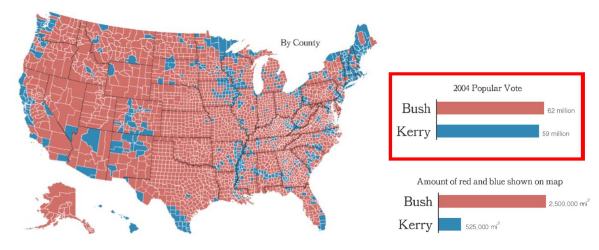
\includegraphics[width=0.5\linewidth]{imgs/lecture8/8.1 choropleth map.png}
    \caption{Choropleth map and message conveying ability}
    \label{fig:8.1}
\end{figure}

\section{Symbol map}
A symbol map, which can be a disk, a square, or a shape, is placed at a point and scaled such that its area is proportional to the quantity associated with the point. We can use area, shape, and color as channels. Unlike a choropleth map, a symbol map avoids confusing geographic areas with data values. One can even use graphs/charts/complex glyphs as symbols, even encoding multiple attributes. \par
A symbol map can be intuitive and easy to understand, they solve the issue of region dimension vs the value of the visualized attribute, because the symbol dimension is proportional to the data value and not to the region dimension. However, when encoding the data using a symbol map, one should try to avoid complex symbols, for they can be harder to understand; and the symbols' placement can be an issue: some symbols can overlap and hide other symbols or even region boundaries.

\begin{figure}[htbp]
    \centering
    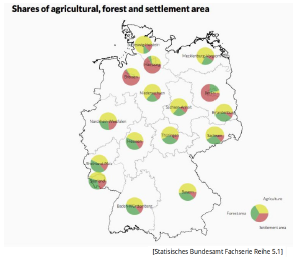
\includegraphics[width=0.3\linewidth]{imgs/lecture8/8.2 symbol map.png}
    \caption{Symbol map}
    \label{fig:8.2}
\end{figure}

\section{Dot density map}
A dot density map typically uses points as marks, and points are positioned over a map, where each dot represents a given constant quantity of items; all dots are equal, it is their quantity and distribution that gives information. \par
A dot density map is easy and intuitive, which mitigates the confusion between region areas and displayed values. But an accurate estimate can be difficult to make, due to the overlap of information and the quantity of dots. Sometimes, the normalization may be needed (for example, 1 dot = number cases / 1000 people).

\begin{figure}
    \centering
    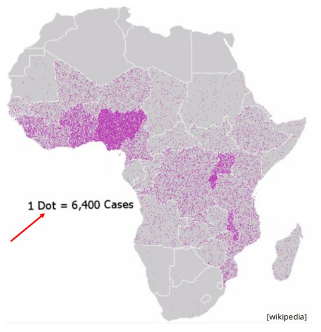
\includegraphics[width=0.3\linewidth]{imgs/lecture8/8.3 dot density map.png}
    \caption{Dot density map}
    \label{fig:8.3}
\end{figure}

\section{Contiguous cartogram}
It is a particular representation of the data where the geographic position and boundaries among regions are preserved, while dimensions are distorted according to a quantitative attribute. The aim is to preserve as much as possible the original position, shape, and boundary, and minimize distortion.

\begin{figure}[htbp]
    \centering
    
    \begin{subfigure}{0.45\textwidth}
        \centering
        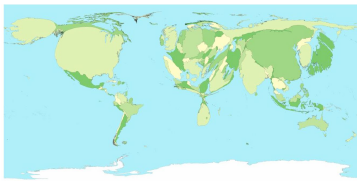
\includegraphics[width=0.6\linewidth]{imgs/lecture8/8.4 contiguous cartogram.png}
        \caption{Contiguous cartogram}
        \label{fig:8.4a}
    \end{subfigure}
    \hfill
    \begin{subfigure}{0.45\textwidth}
        \centering
        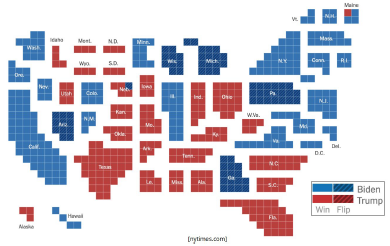
\includegraphics[width=0.6\linewidth]{imgs/lecture8/8.5 grid cartogram.png}
        \caption{Grid variation}
        \label{fig:8.4b}
    \end{subfigure}

    \caption{Contiguous cartogram and its grid variant}
    \label{fig:8.4}
\end{figure}

\section{Best practice - ten rules}
There are some recommended best practices that one should keep in mind when choosing a visualization tool. The ten rules are: best channel first; ensure accuracy and transparency; no unjustified 2D; no unjustified 3D; eyes beat memory; overview first, zoom and filter, details on demand; responsiveness is required; pay attention to color; function first, form next; self-contained visualizations

\subsection{Best channels first}
Recall the \textit{effectiveness principle}: the relevance of information displayed should match the effectiveness of the channel. Meaning that the relevant information should be prioritized, then encoded with the most effective/accurate channels. \par
We have seen channel rankings; to follow this rule means to use the highest-ranked channels for the most important attributes, and the other channels for the remaining, secondary attributes.

\subsection{Ensure accuracy and transparency}
Recall the expressiveness principle: the visual representation should represent all of, and only, the relationships that exist in the data. This implies that information that is not present in the data should not be visualized. It is also important to not to convey misleading information while paying attention to axis starting values and scale, and align data when possible for accurate comparisons, and more.

\subsection{No unjustified 3D}
Misconception: \textit{if two dimensions are good, then three dimensions must be better}. \par
There are many difficulties in visually encoding information with the third spatial dimension, depth. 3D visualization is justified only when the user's task involves shape understanding of inherently three-dimensional structures; usually, these inherently spatial data are scientific visualization and computer graphics, where the use of 3D is fundamentally required for understanding the three-dimensional geometric structure of objects or scenes. In all other contexts, the use of 3D needs to be carefully justified. \par

\begin{figure}[htbp]
    \centering
    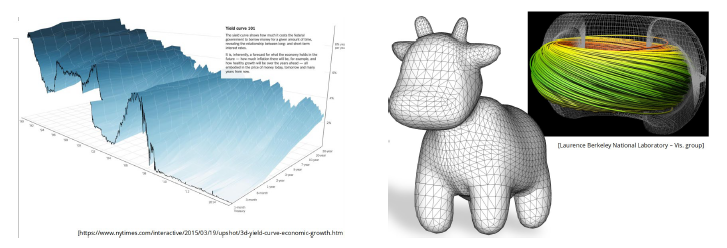
\includegraphics[width=0.5\linewidth]{imgs/lecture8/8.6 justified 3d.png}
    \caption{Justified 3D use cases}
    \label{fig:8.5}
\end{figure}

One of the main issues is occlusion, where some objects cannot be seen because they are hidden behind others. The overarching problem with occlusion in the context of visual encoding is that presumably important information is hidden (the occluded detail might even be critical), and discovering hidden details via navigation has a time cost.\par
In visually encoding abstract data, perspective is another very bad thing. Perspective distortion is one of the main dangers of depth because the power of the plane is lost; it completely interferes with visual encoding that uses the planar spatial position channels and the size channel, e.g., it is more difficult to judge and compare bar heights in a 3D bar chart than in multiple horizontally aligned 2D bar charts. \par
Another problem with the use of 3D is dramatically impaired text legibility. Text fonts have been very carefully designed for maximum legibility when rendered on the grid of pixels that makes up a 2D display. Text tilted in any way off the image plane typically becomes jaggy.

\begin{figure}[htbp]
    \centering
    
    \begin{subfigure}{0.45\textwidth}
        \centering
        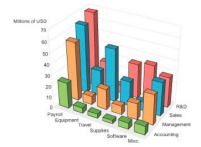
\includegraphics[width=0.6\linewidth]{imgs/lecture8/8.7 unsjustified 3d.png}
        \caption{Perspective issue}
        \label{fig:8.6a}
    \end{subfigure}
    \hfill
    \begin{subfigure}{0.45\textwidth}
        \centering
        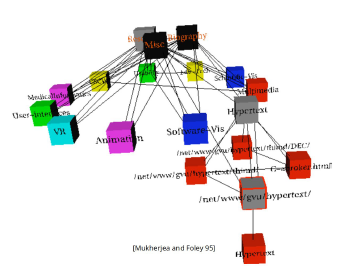
\includegraphics[width=0.6\linewidth]{imgs/lecture8/8.8 unjustified 3d.png}
        \caption{Text legibility issue}
        \label{fig:8.6b}
    \end{subfigure}

    \caption{Unjustified 3D use cases}
    \label{fig:8.6}
\end{figure}

\subsection{No unjustified 2D}
Laying out data in a 2D space should be explicitly justified, compared with the alternative of simply showing the data with a 1D list.

\subsection{Eyes beat memory}
Using our eyes to switch between different views that are visible simultaneously has a much lower cognitive load than consulting our memory to compare a current view with what was seen before. \par
The phenomenon of change blindness is that we fail to notice even quite drastic changes if our attention is directed elsewhere. Although we are very sensitive to changes at the focus of our attention, we are surprisingly blind to changes when our attention is not engaged. The difficulty of tracking complex and widespread changes across multi-frame animations is one of the implications of change blindness for visualization.\par
In simpler words, seeing lasts longer than remembering, but distraction prevents us from noticing changes.

\subsection{Overview first, zoom and filter, details on demand}
This is a visualization idiom that provides an overview is intended to give the user a broad awareness of the entire information space with the goal of summarizing. An overview helps the users to find regions where further investigation in more detail might be productive. An overview is often shown at the beginning of the exploration process to guide users in choosing where to drill down to inspect in more detail.

\subsection{Responsiveness is required}
The latency of interaction, namely, how much time it takes for the system to respond to the user action, matters immensely for interaction design. Human reaction to phenomena is best modeled in terms of a series of discrete categories, with a different time constant associated with each one. A system will fell responsive if these latency classes are taken into account by providing feedback to the user within the relevant time scale. \par
From a user's point of view, the latency of an interaction is the time between their actions and some feedback from the system indicating that the operation has completed. In a visualization system, that feedback would most naturally be some visual indication of state change within the system itself. The user should have some sort of confirmation that the action has completed. If an action could take significantly longer than a user would naturally expect, at least some kind of progress indicator should be shown to the user. 

\subsection{Pay attention to color}
The use of color should be justified, because there are higher-ranked channels than color. Items should be easy to tell apart by using contrast. A limited number of available hues and a limited number of bins should be used (avoid similar colors). Take into consideration color blindness. \par
Hue for categorical attributes, saturation, and luminance for attributes for which ordering is meaningful.
\subsubsection{Get it right in black and white}
It is a design guideline for effective use of color, ensuring that the most crucial aspect of visual representation is legible even if the image is transformed from full color to black and white. This suggests encoding the most important attribute with the luminance channel to ensure adequate luminance contrast, and considering the hue and saturation channels as secondary sources of information. 

\subsection{Function first, form next}
The best visual design should be both beautiful and effective; however, given an effective but ugly design, it is possible to refine the form to make it more pleasing while maintaining the base of effectiveness. In contrast, given a pleasing but ineffective design, you will probably need to toss it out and start from scratch since progressive refinement is not possible. \par
Visual beauty does matter, given that visualization makes use of human visual perception. Good visual form enhances the effectiveness of visual representations. 

\subsection{Self-contained visualizations}
Look at the visualization, which should be enough to understand the visualization itself. The labels, titles, legends, and descriptions can be added if needed, but if more information is required for understanding the visualization, one should rethink the design.
\chapter{Lecture 9 - Multidimensional data}

\begin{figure}[htbp]
    \centering
    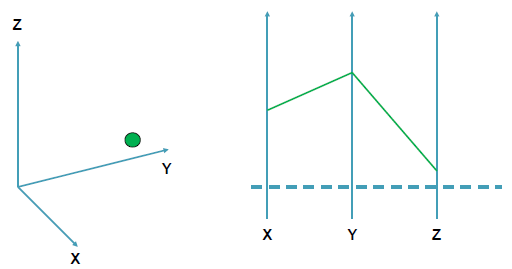
\includegraphics[width=0.3\linewidth]{imgs/lecture9/9.1 parallel coordinates.png}
    \caption{Parallel coordinates and cartesian coordinates}
    \label{fig:9.1}
\end{figure}
Parallel coordinates can be used to visualize multivariate data as an extension of Cartesian coordinates. Note that the order of the axes plays a fundamental role in its readability. 

Together with parallel coordinates, scatterplot matrices can be used to represent multidimensional data (among other visualization tools). However, a different approach exists, which is to \textit{reduce the dimensionality} of the data. This is a widely used strategy to map the dimensionality of the dataset from a higher N-dimension to 2 or 3 dimensions for a better understanding. Note that dimensionality reduction is a mapping, not a geometric transformation. It has different techniques, each with different properties.

\section{PCA - Principal Component Analysis}
PCA is a linear, non-parametric multidimensional reduction technique. The core idea is to find a basis formed by the directions that maximize the variance of the data, so that it can express the data in a new basis that best expresses our dataset. \par
Mathematically, if \(X\) is our original dataset and \(P\) is the transformation matrix, the new data \(Y\) is obtained as \(Y = XP\). In this transformation, each row of \(P(p_1, \dots ,p_m )\) represents a new direction (principal component), and \(Y\) represents the projection of the original data onto these directions

\begin{equation}
    \label{eq:9.1}
    PX = 
    \begin{bmatrix}
        \mathbf{p}_1 \\
        \vdots \\
        \mathbf{p}_m
    \end{bmatrix}
    [\mathbf{x}_1 \ \ldots \ \mathbf{x}_n]
\end{equation}

\subsubsection{Covariance Matrix}
The role of the covariance matrix is to find the best directions. PCA looks at the covariance Matrix (\(C_X\)) of the original data such that \(C_X = 1/(n-1)XX^T\), where the diagonal terms represent the variance of every single variable, while off-diagonal terms represent the covariance (redundancy) between different variables.\par
The goal is to find a matrix \(P\) such that the covariance matrix of the transformed data (\(C_Y\) is diagonalized, in other words, a matrix \(P\) that maximizes the variance and minimizes the redundancy. 
\begin{itemize}[noitemsep]
    \item Maximize variance implies that high values on the diagonal mean the dynamics of the variables are captured effectively.
    \item Minimize redundancy implies that the low off-diagonal values mean variables are no longer redundant.
\end{itemize}

\subsubsection{Solving PCA}
\begin{theorem}
    A symmetric matrix \(A\) can be diagonalized by a matrix formed by its eigenvectors as \(A = EDE^T\), where the columns of \(E\) are the eigenvectors of \(A\).
\end{theorem}

The solution relies on Theorem 9.1. The steps to compute PCA are:
\begin{enumerate}[noitemsep]
    \item Organize data as a \(m \times n\) matrix
    \item Subtract the mean from each row
    \item Calculate the eigenvalues and eigenvectors of \(XX^T\)
    \item The eigenvectors organized by their corresponding eigenvalues from the matrix \(P\)
\end{enumerate}

Remember that \(Y=PX\), we define the covariance matrix of the new data \(C_Y = 1/(n-1)YY^T\)
\begin{enumerate}[noitemsep]
    \item substitute \(Y\) with \(PX\): \(= 1/(n-1)(PX)(PX)^T\)
    \item resolve the equation: \(= 1/(n-1)PXX^TP^T\)
    \item apply the theorem 9.1: \(= 1/(n-1)P(XX^T)P^T\)
    \item as the result of Theorem 9.1, we obtain that \(C_Y = 1/(n-1)PAP^T\), where \(P\) is transformation matrix and \(A\) is the symmetric matrix
\end{enumerate}

\subsubsection{Reducing dimensionality and reconstruction error}
Reduction occurs when we choose only the first \(k\) principal components (\(k < m\)). By projecting the data onto these \(k\) directions, we get a lower-dimensional representation that is the best approximation of the original data. \par
PCA minimizes the reconstruction error \(e\), defined as the sum of squared differences between the original points (\(y_i\)) and the projected points (\(\tilde{y_i}\)):

\begin{equation}
    \label{eq:9.2}
    e = \sum_i^k(\tilde{y_i} - y_i)^2
\end{equation}

In fig. \ref{fig:9.2} shows a visual example of a ball attached to a spring moving along a single axis (the x-axis). If three different cameras record this movement, the raw data has 6 dimensions (x, y, coordinates for each of the 3 cameras). Because the ball only moves in 1D, most of these 6 dimensions are redundant or contain noise, but applying PCA allows the system to identify the single primary direction of motion, effectively reducing 6 noisy dimensions back to the 1 meaningful dimension that captures the most variance.
\begin{figure}[htbp]
    \centering
    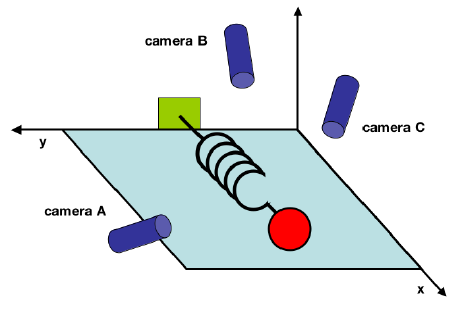
\includegraphics[width=0.5\linewidth]{imgs/lecture9/9.2 PCA example.png}
    \caption{visual example of PCA dimensionality reduction}
    \label{fig:9.2}
\end{figure}

\subsubsection{Limitations}
\begin{itemize}[noitemsep]
    \item Non-parametric: while a strength, it can be a weakness because it does not incorporate prior knowledge
    \item distribution: it fails for data that is not Gaussian-distributed
    \item linearity: it is a linear technique; for non-linear structures, extensions like kernel PCA or other methods are needed
    \item independence: PCA does not guarantee statistical independence
\end{itemize}

\section{MDS - Multi-Dimensional Scaling}
MDS is a classic technique for dimensionality reduction. The primary rationale behind MDS is to find a lower-dimensional representation of data that preserves the pairwise distances between points as accurately as possible.
\begin{itemize}
    \item The mapping: it seeks a linear mapping (\(y_i = Mx_i\)) that minimizes a cost function (\(\phi(Y)\)) representing the differences between the Euclidean distance of points in the high-dimensional space (\(d_{ij}^2\)) and their distance in the low-dimensional space (\(||y_i - y_j||^2\))
    \begin{equation}
        \phi(Y) = \sum_{i, j} d^2_{ij} - || y_i - y_j||^2
    \end{equation}
    \item relationship to PCA: minimizing the distance mismatch (\(\phi(Y)\)) is mathematically equivalent to maximizing the variance of the points in the new space, which is the exact goal of PCA.
\end{itemize}

\subsubsection{MDS vs PCA}
While the two techniques share similar goals and both better preserve large pairwise distances, they differ significantly in their computational scaling:
\begin{itemize}
    \item PCA scales based on the dimensions of the data (the size of the covariance matrix is proportional to the number of variables)
    \item MDS scales based on the number of data points. This makes MDS a distinct choice depending on whether a dataset has many variables or many individual samples.
\end{itemize}

\subsubsection{Sammon mapping variant}
It is a specific adaptation of MDS that allows for retaining the local structure of the data better than classical MDS, where retention of high distances is privileged, and not of local structure. Sammon mapping addresses this by weighting the contribution of each pair of points.

\section{LLE - Locally Linear Embedding}
LLE is a dimension reduction technique designed to discover non-linear structures in high-dimensional data by exploiting local linear approximations. While PCA is a linear technique that looks at global variance. LLE operates on the intuition that even if a dataset is globally non-linear, it can be approximated as locally linear.

\subsubsection{Core intuition}
The fundamental assumption of LLE is that the high-dimensional data lies on a "well-sampled" manifold. Because the manifold is well-sampled, any given data point and its immediate neighbors can be treated as a small, locally linear patch. Each point in this patch can be represented as a weighted sum of its neighbors.

\subsubsection{The LLE algorithm}
LLE follows a three-step mathematical process to map high-dimensional points into a lower-dimensional space:
\begin{enumerate}[noitemsep]
    \item \textbf{identify neighbors}: for every data point \(X_i\) in the high-dimensional space, the algorithm finds its K-nearest neighbors or all points within a specific ball radius.
    \item \textbf{compute reconstruction weights}: the algorithm calculates the weights \(W_{ij}\) that best reconstruct each point \(X_i\) from its neighbors by minimizing the error function: 
    \begin{equation}
        \label{eq:9.3}
        \epsilon(W) = \sum_i | X_i - \sum_j W_{ij} X_j|^2
    \end{equation}
    In this step, the weights capture the local geometric properties of the data
    \item \textbf{map to low-dimensional space}: finally, the algorithm finds new vectors \(Y_i\) in a lower-dimensional space (2D or 3D) that respect those same weights. It does this by minimizing a new cost function while keeping the weights \(W_{ij}\) fixed:
    \begin{equation}
        \label{eq:9.4}
        \Phi(Y) = \sum_i |Y_i - \sum_j W_{ij}Y_j|^2
    \end{equation}
    This ensures that the local neighborhood relationships from the original high-dimensional space are preserved in the new, reduced space.
\end{enumerate}

\section{Isomap}
The Isomap is a dimensionality reduction technique based in the core principle of preserving the geodesic distance between data points. It is designed to understand the intrinsic geometry of a curved space (a manifold).\par
In a high-dimensional space where data lies on a curved surface, the straight-line Euclidean distance between two points can be misleading because it "cuts through" the empty space of the manifold.
\begin{definition}[Geodesic Distance]
    Geodesic distance is the shortest path between two points measured along the surface of the curved space.
\end{definition}
An isomap aims to "unroll" this curved manifold into a flat representation while keeping the distances along the surface consistent.

\subsubsection{Procedure}
The Isomap algorithm can be seen as a three-step mathematical procedure:
\begin{enumerate}[noitemsep]
    \item \textbf{construct neighborhood graph (\(G\))}: define a graph over all data points by connecting all points (i, j) if and only if point \(i\) is one of the K-nearest neighbors of point \(j\)
    \item \textbf{compute the shortest path}: using Floyd's algorithm (or a similar shortest-path algorithm) to calculate the shortest path between all pairs of points in the graph \(G\). This results in an approximation of the global geodesic distances between all points in the dataset.
    \item \textbf{construct the d-dimensional embedding}: use the matrix of approximated geodesic distances to find a lower-dimensional representation.
\end{enumerate}

\subsubsection{Applications}
Isomap is particularly effective for datasets where the "meaningful" dimensions are non-linear:
\begin{itemize}[noitemsep]
    \item Face poses: when applied to a dataset of faces, Isomap can successfully map images onto axes representing "up-down pose" and "left-right pose", capturing the natural rotation of a head
    \item Handwriting: Isomap can be used to visualize how different digits vary based on their "top arch" or "bottom loop" articulation
\end{itemize}

\section{Autoencoder}
An autoencoder is a specialized type of neural network used to perform dimensionality reduction. These networks offer a powerful way to map complex data into simpler forms. A multi-layer autoencoder consists of two primary components that work together to process data:
\begin{itemize}[noitemsep]
    \item The \textbf{encoder} that takes the high-dimensional \textbf{input data X}, and passes it through several layers of neurons. Each layer uses a set of weights to progressively compress the information. 
    \item At the center of the network is a \textbf{"bottleneck" layer}. This layer holds the compressed, \textbf{low-dimensional representation (Y)} of the input data, effectively capturing its most essential features
    \item The \textbf{decoder} performs the reverse operation of the encoder by using a mirrored set of transposed weights to attempt to reconstruct the original data from the compressed representation. Thus, obtaining the final \textbf{output data X'}
\end{itemize}

\begin{figure}[htbp]
    \centering
    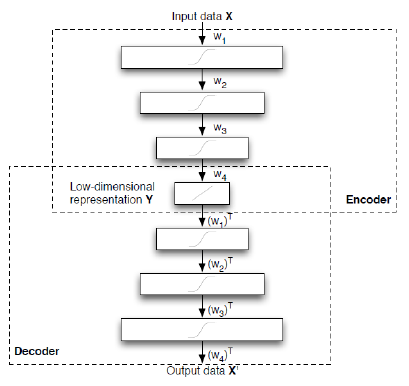
\includegraphics[width=0.4\linewidth]{imgs/lecture9/9.3 autoencoder.png}
    \caption{Multi-layer autoencoder}
    \label{fig:9.3}
\end{figure}

The network is trained to ensure that the output data X' is as close to the input data X as possible. Because the data must pass through the low-dimensional bottleneck Y, the autoencoder is forced to learn a highly efficient way to represent the data. \par
To make it work for dimensionality reduction, once the network is trained, the decoder part can be discarded, and the encoder can be used as a tool to transform high-dimensional datasets into a 2D or 3D representation for visualization and analysis, similar to the goals of PCA or Isomap.

\section{t-SNE}
t-SNE stands for t-Distributed Stochastic Neighbor Embedding, a state-of-art dimensionality reduction technique to a common problem: the inability of most techniques to retain both local and global structure of data in a single 2D or 3D map.

\subsection{SNE}
Before introducing t-SNE, it is important to understand its predecessor. SNE models the relationships between data points using conditional probability rather than fixed distances. 
\begin{itemize}
    \item High-dimensional similarity (\(p_{j|i}\)): in the original high-dimensional space, the similarity of point \(x_j\) to point \(x_i\) is the probability that \(x_i\) would pick \(x_j\) as its neighbor. This is calculated using a Gaussian distribution centered at \(x_i\)
    \item Low-dimensional similarity (\(q_{j|i}\)): an analogous probability is calculated for the points in the lower-dimensional space
\end{itemize}
The objective is to ensure that the low-dimensional map Q reflects the high-dimensional neighborhood structure P as closely as possible, i.e., minimizes the mismatch between \(p_{j|i}\) and \(q_{j|i}\), this can be achieved using the KL divergence.

\subsection{Kullback-Leibler (KL) Divergence}
To quantify how much the low-dimensional map differs from the original data, SNE uses KL Divergence, also known as relative entropy.
\begin{itemize}
    \item Coding theory view: it represents the expected number of extra bits required to code samples from distribution \(P\) if the code is optimized for distribution \(Q\).
    \item Bayesian view: it measures the information gained when one revises beliefs from a prior distribution Q to a posterior distribution P.
    \item Mathematical property: a critical detail noted in the sources is that KL divergence is not symmetric, meaning \(KL(P||Q) \neq KL (Q||P)\).
\end{itemize}

\subsection{Into t-SNE}
Standard SNE has two major flaws: its cost function is difficult to optimize, and it suffers from the "crowding problem", where points in the low-dimensional map tend to collapse together into a cluttered center. t-SNE solves these through two specific innovations:
\begin{itemize}[noitemsep]
    \item \textbf{Symmetry}: t-SNE makes the SNE cost function symmetric, which simplifies the optimization process \(KL(P||Q) = KL (Q||P)\)
    \item \textbf{Student-t distribution}: instead of the Gaussian distribution, t-SNE uses the Student-t distribution with one degree of freedom to evaluate similarities in the low-dimensional space. The "heavy tails" of the Student-t distribution allow points that are far apart in the high-dimensional space to be modeled as even farther in the low-dimensional space, which effectively alleviates the crowding problem.
\end{itemize}
\chapter{Lecture 10 - Data Visualization in Python}
Python is a perfect glue between several data manipulation tools, scientific libraries, and visualization toolkits. It is easy to learn and is a continuously supported language by the computer scientist community.

\section{NumPy}
NumPy is a specialized Python tool that Python has for efficient storage and manipulation of numerical arrays. NumPy arrays are like a built-in list type, but the tool supports efficient storage and data operations as the array grows larger in size.\par
A Python list is a data structure containing a reference count, a data type, the size in bytes, and the content. Hence, a Python list is a pointer to a block of pointers, which makes it flexible at the cost of efficiency.\par
On the other hand, a NumPy array is a fixed-type ndarray containing non-redundant information, which allows high efficiency in terms of memory and processing with reduced flexibility. 

\subsection{NumPy array manipulation}

\subsubsection{Array slicing}
\begin{itemize}[noitemsep]
    \item accessing a single element: A[3, 2], denote the element at the 3rd row and 2nd column
    \item slicing: A[start, stop, step]
    \item first 5 elements: A[:5]
    \item elements from index 5: A[5:]
    \item sub-array: A[3:8]
\end{itemize}

\subsubsection{Sub-arrays as no-copy views}
Slicing operations on an ndarray return a view, not a copy of the array data. If we modify the sub-array, the corresponding part of the array would be updated. To create a copy of the sub-array, an explicit \textit{copy()} method needs to be called. \par
Example: \par
--> x\_sub = x[:2, :2].copy()

\subsubsection{Reshaping}
The \textit{reshape()} method is used to change the array structure. \par
Example: \par
--> x.shape() returns (6, 3), a 6x3 matrix \par
--> y = x.reshape (18, 1) \par
--> y.shape() returns (18, 1),  a 18 elements vector

\subsubsection{Concatenation and Splitting}
\textit{Concatenation()} method concatenate two or more arrays or other methods such as \textit{vstack()} for vertical stacking (rows) and \textit{hstack()} for horizontal stacking (columns).\par
Analogously, an ndarray can be split using methods like \textit{split()}, \textit{hsplit()} and \textit{vsplit()}

\subsection{ndarray computations}
Standard Python loops, such as the \textit{for} loop, are extremely slow for elaborating a large quantity of numerical data. This is because Python is a runtime compiled language. \par
However, NumPy provides an interface for this kind of statically typed compiled runtime using vectorized operations.\par
Universal Functions or Ufuncs are the vectorized operations in NumPy, which execute element-wise operations with low latency. Some examples include: arithmetic operations (+, -, *, /); absolute values, trigonometric functions (sin, cos); exponents and logarithms; and specialized functions.

\subsection{Broadcasting}
Broadcasting is a set of rules that allow NumPy to execute operations between arrays and matrices of different sizes without creating redundant copies in memory, thus avoiding explicit loops and storage inefficiency. It has fundamentally three rules:
\begin{enumerate}[noitemsep]
    \item If the two arrays differ in their number of dimensions, the shape of the one with fewer dimensions is padded with ones on its leading (left) side
    \item  if the shape of the two arrays does not match in any dimension, the array with shape equal to 1 in that dimension is stretched to match the other shape
    \item if in any dimension the size disagrees and neither is equal to 1, an error is raised 
\end{enumerate}

\begin{figure}[htbp]
    \centering
    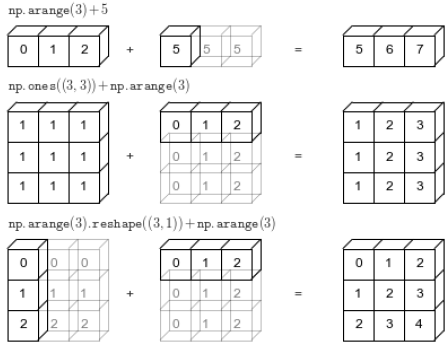
\includegraphics[width=0.5\linewidth]{imgs/lecture10/10.1 broadcasing.png}
    \caption{Broadcasting rules explained}
    \label{fig:10.1}
\end{figure}

\section{Pandas}
Pandas is an open-source library that provides high-performance, easy-to-use data structures and analysis tools. Its primary objects, \textit{Series and DataFrames}, are built on top of NumPy arrays to provide both the flexibility needed for data wrangling (like handling labeled data) and the efficiency of numerical arrays. 

\subsection{Series}
A Series is defined as a one-dimensional array of indexed data. While a NumPy array defines an implicit integer index, a Pandas Series allows for an explicitly defined index. A Series can also be thought of as a specialized type of dictionary where keys are the indices and values are the data points. \par
Examples: \par
--> data = pd.Series ([a, b, c, d], index=[1, 2, 5, 7])\par
--> data[5] returns \textit{c}

\subsection{DataFrame}
While a Series is 1D, a DataFrame is a two-dimensional array with flexible row indices and flexible column names. It can be viewed as a sequence of aligned Series objects that share the same index.

\subsection{Indexing and Selection}
Pandas can sometimes be ambiguous when using integer indices \par
--> Is data[5] refers to the explicit label or the implicit fifth position?\par
To solve this, the library provided specific indexer attributes:
\begin{itemize}[noitemsep]
    \item \textbf{loc}: always refers to the \textbf{explicit} index (the user-defined label)
    \item \textbf{iloc}: always refers to the \textbf{implicit} index (the Python-style positional index starting from 0)
    \item \textbf{ix}: a hybrid of the two, though less commonly used in the modern versions.
\end{itemize}
Examples: \par
--> data = pd.Series ([a, b, c, d], index=[1, 2, 5, 7])\par
--> data.loc[1] returns \textit{a}\par
--> data.iloc[1] returns \textit{b} \par
--> data.loc [1:2] returns {[1, a], [2, b]} \par
--> data.iloc[1, 2] returns {[2, b], [5, c]} \par
One can access the column name in a dictionary-style (--> data['population']) or in an attribute-style (--> data.population). However, the assignment works only for a dictionary-style.

\subsubsection{Indexing conventions for DataFrame}
While indexing refers to columns, slicing refers to rows. Also direct masking operations are interpreted row-wise rather than column-wise.\par
--> data[data.density > 100] returns rows of the dataframe that satisfies the condition\par
Ufuncs preserve index and column labels in the output, and for binary operations like addition and multiplication, Pandas automatically align indices.

\subsection{Handling missing data}
Pandas is particularly robust at managing "junk" or missing data. It uses \textit{None} for generic object data and \textit{NaN} for numerical values. It can automatically convert between these types when appropriate (if inserting None into an integer array will convert the array to floating-point and use NaN). \par
It offers built-in methods to work on missing data, either to fill in, to remove, or to replace. For example, \textit{dropna()}, which can remove missing values from a Series or entire rows/columns from a DataFrame.

\section{Data visualization tools in Python}
Python offers a vast and interconnected landscape of visualization libraries. At the heart is Matplotlib, which serves as the foundation for many other popular tools like Seaborn and the built-in plotting functions in Pandas. Other libraries include JavaScript-based tools like Plotly and Bokeh, and OpenGL-based tools for high-performance rendering. 

\subsubsection{Matplotlib}
This library is heavily inspired by Matlab, making it very easy for researchers moving from that environment to adapt. 

\begin{itemize}[noitemsep]
    \item \textbf{Pros}: It is extremely flexible and supports many different rendering backends
    \item \textbf{Cons}: The API is imperative (you need to tell it exactly how to draw every piece), the default style is considered poor, and it lacks interactivity; it can be slow when handling very large datasets or complex designs
\end{itemize}

\subsubsection{Matplotlib inspired tools}
\begin{itemize}[noitemsep]
    \item \textbf{Pandas}: Its goal is to provide a simple way to visualize a DataFrame directly, often including more complex graphs with less code than raw Matplotlib
    \item \textbf{Seaborn}: This library is specifically targeted toward statistical data visualization. It provides much aesthetically pleasing default "nice style" and simplifies the creation of complex plots, such as joint plots that combine scatter plots with histograms or kernel density estimates.
\end{itemize}

\subsubsection{Plotly}
It is a modern alternative to the Matplotlib family, built on JavaScript. It provided high interactivity, allowing users to zoom, hover for data, and toggle categories. While it uses JavaScript for the rendering, a version called Dahs is available that allows Python users to build interactive dashboards without needing to write any JavaScript code.

\subsubsection{Imperative vs Declarative}
Imperative means that you have to manually specify the graphs and the related details.\par
Declarative means that you have to specify what should be done with the data, and the framework decides the details.
\chapter{Lecture 11 - Graph drawing}

\begin{definition}[graph drawing]
    Graph drawing is the process of taking an abstract graph \(G = (V, E)\), consisting of a set of vertices (V) and a set of edges (E), and using an algorithm to produce a visual "drawing". 
\end{definition}

Graph drawing is essential across many scientific and technical fields where relationships between entities need to be visualized. For instance, in engineering, it is used for designing electric circuits; in computer science, it helps in website analysis and visualizing computer networks; in social and security science, the emerging applications include intelligent analysis, forensic accounting, and more.\par
Graph drawing is closely linked to several other fields: graph theory (mathematical properties of graphs), information visualization (using visuals to explore abstract data), computational geometry (solving geometric problems using computers), and algorithm engineering (devising efficient computational processes). \par

\section{Planarity}

\begin{definition}[Planar embedding]
    Planar embedding is a way to map the graph to a 2D plane such that no edges intersect
\end{definition}

The primary challenge in graph drawing is to find a planar embedding. To simplify the problem, it is suggested to break the graph down based on its connectivity:
\begin{itemize}[noitemsep]
    \item cut-vertex: a specific vertex whose removal produces a disconnected graph
    \item bi-connected graph: a graph that contains no cut-vertices
    \item blocks: you can recursively split a graph into smaller bi-connected pieces, which are called blocks
    \item Block-Cut-vertex Tree (BC-tree): the relationships between these blocks and the cut-vertices used to split them are represented by a specialized tree structure
\end{itemize}

\begin{theorem}[Planarity]
    A graph is planar if and only if all of its individual blocks are planar
\end{theorem}
Thanks to this theorem, which allows researchers to use a divide-and-conquer strategy: instead of testing a massive, complex graph all at once, you can test each block separately.

\subsection{The Auslander and Parter algorithm}
It is an established algorithm with computational cost of \(O(n^2)\), a method for planarity testing. 
\begin{enumerate}[noitemsep]
    \item \textbf{Bi-connectivity assumption} --> the algorithm assumes the input graph is bi-connected. If the graph is not bi-connected, the divide-and-conquer strategy can be used to test its individual blocks one by one.
    \item \textbf{Selecting a cycle and identifying "pieces"} --> the process begins by finding a cycle C within the graph, and the algorithm identifies the "pieces" attached to C. A \textbf{piece} can be a single edge connecting two non-consecutive vertices on the cycle, or a more complex subgraph connected to the cycle at specific points. Every piece must eventually be drawn either entirely inside or entirely outside the cycle C to avoid crossing edges
    \item \textbf{Building the incompatibility Graph} --> the algorithm builds a secondary graph, called the incompatibility graph, to determine if a piece can be placed without crossing. Each node in such a graph represents one of the pieces identified in the previous step. An edge is drawn between two nodes if their corresponding pieces conflict. A conflict occurs if the two pieces cannot be placed on the same side of the cycle without crossing each other
    \item \textbf{Bipartite-ness} --> once the incompatibility graph is built, the algorithm checks if it is bipartite. A graph is \textbf{bipartite} if the pieces can be partitioned into two groups, those that are drawn inside the cycle and those that are drawn outside. If it is not bipartite, it means that the graph contains a cycle of conflict that makes it impossible to draw it without at least one crossing. In this case, the graph is non-planar
    \item \textbf{Divide-and-Conquer recursion} --> passing the incompatibility test for each cycle is not enough. The algorithm must ensure that the internal structure of each piece is also planar. The algorithm repeats the entire process recursively for each piece, combined with the cycle it is attached to. The recursion stops when a piece is reduced to a simple path or a single edge, at which point it is inherently planar.
\end{enumerate}

\section{Graph drawing aesthetics}
While an algorithm can produce many different drawings of the same graph, not all of them are equally useful. Aesthetics can be seen as mathematical properties that correlate with the readability of a drawing.

\subsubsection{Minimizing crossing}
The most fundamental aesthetic is reducing the number of edge intersections. A drawing is clearer if the number of intersections is reduced. This is why planarity testing is so critical. A planar drawing (no crossings) is generally the gold standard for readability.

\subsubsection{Minimizing size (area)}
A good drawing should be compact. Small size allows the user to see a large picture of the drawing at once. One should try to minimize the total area of the drawing, the maximum edge length, and the average edge length.

\subsubsection{Minimizing bends}
In certain drawing conventions (like "orthogonal" drawings where edges are made of horizontal and vertical segments), edges can have "bends" or angles. Edges with many bends are difficult to follow for human eye.

\subsubsection{The contrast of aesthetics}
A crucial insight is that these aesthetics often conflict with each other. You cannot always minimize everything at once. Choosing the "best" drawing often involves a trade-off between these competing goals

\subsubsection{drawing conventions}
When an algorithm is tasked with creating a drawing, it must follow a drawing convention, a set of geometric rules that define the style and constraints of the output.
\begin{itemize}[noitemsep]
    \item Polyline: edges are represented as a sequence of connected line segments
    \item Straight line: edges are simple, single straight segments between vertices
    \item Layered: vertices are arranged into horizontal layers, often used for hierarchical structures
    \item Orthogonal: edges are made up only of horizontal and vertical segments
\end{itemize}
Drawing on the grid can ensure precision and help minimize the total area of the drawing. In a grid drawing, vertices are required to have integer coordinates. This approach helps satisfy the aesthetic goal of small size, which allows users to see more of the graph at once. 

\section{Kuratowski's theorem}
While many graphs can be drawn planarly, others are inherently non-planar. The Kuratowski theorem provides criteria for identifying these graphs

\subsubsection{The minimal non-planar graphs}

\begin{figure}[htbp]
    \centering
    
    \begin{subfigure}[b]{0.45\textwidth}
        \centering
        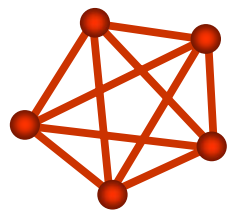
\includegraphics[width=0.4\linewidth]{imgs/lecture11/11.1 non-planar.png}
        \caption{}
        \label{fig:11.1a}
    \end{subfigure}
    \hfill
    \begin{subfigure}[b]{0.45\textwidth}
        \centering
        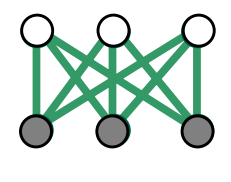
\includegraphics[width=0.4\linewidth]{imgs/lecture11/11.2 non-planar.png}
        \caption{}
        \label{fig:11.1b}
    \end{subfigure}

    \caption{Non-planar drawings}
    \label{fig:11.1}
\end{figure}

The two minimal non-planar graphs: there are two specific structures that make a graph non-planar. Fig \ref{fig:11.1a} is a complete graph with 5 vertices where every vertex is connected to every other vertex. Fig \ref{fig:11.1b} is a complete bipartite graph where two sets of three vertices are connected to each other, also known as the "utility graph"

\subsubsection{The subdivision rule}
A graph does not have to be exactly one of the two drawings in fig. \ref{fig:11.1} to be non-planar; it only needs to contain a subdivision of one of them. A subdivision occurs when new vertices are inserted along the edges of the original structure.
\include{lectures/lecture12}
\chapter{Lecture 13 - 3D data representation}

3D data is used across a vast array of fields, including cultural heritage, medicine, architecture, and security. It highlights that 3D models are no longer just for animation or gaming; they are critical for digital fabrication, archaeology, and eHealth. \par
There are four primary ways that 3D models are created:
\begin{itemize}[noitemsep]
    \item \textit{Manual modeling}: using dedicated SW like Blender
    \item \textit{Simulation}: generating models through computational physics or biological data
    \item \textit{Acquisition techniques}: using laser scanning or photogrammetry to digitize real-world objects. These techniques has overcome the modeling bottleneck, making 3D creation easier and less expensive.
    \item \textit{Generative AI}: emerging perspectives allow for image-to-3D or text-to-3D generation
\end{itemize}    

Once a model is acquired or created, it enters the \textbf{Geometry Processing} phase. This discipline is concerned with the mathematical models used to represent geometric data and the algorithms used to analyze, manipulate, and smooth that data to remove noise or reduce complexity.

\section{Surface representation}
\begin{definition}[Surface]
    In computer graphics, a surface is intuitively defined as a \emph{2D region within a 3D space} that has length and breadth but no thickness. If the surface is closed, it acts as the boundary of a 3D volume.
\end{definition}

There are two primary mathematical ways to define a surface analytically:
\begin{itemize}[noitemsep]
    \item Implicit surface is defined by an equation \(f(x, y, z) = 0\). As an example, the surface of a sphere, which is defined as \(x^2 + y^2 + z^2 - r^2 = 0\)
    \item Parametric surface is defined by a function mapping a 2D domain into 3D space. This uses coordinates (u, v) to determine the (x, y, z) position of every point on the surface.
\end{itemize}

While the analytical models are precise, they are \textit{difficult to apply to complex, real-world objects}. Consequently, computer graphics relies on discrete representations, which treat complex shapes as collections of simple "building blocks" glued together. The four most common blocks are \textbf{voxels, points, triangles, and quads}.

\subsubsection{Voxels - Volumetric representation}
This method considers a surface as the boundary of a solid volumetric object. It defines an \textbf{indicator function} that maps the 3D domain into a discrete binary domain where \textit{1 means solid and 0 means void}. \par
Alternatively, \textbf{signed distance fields} are a more advanced version that store the distance to the nearest surface at every point in a voxel grid. This provides more information than a simple occupancy map but requires more storage.\par
These are frequently used for massive 3D models, medical data (MRI/CT scans), and physics simulations.\par
This representation is excellent in tasks like rendering applications or volumetric field processing. They break down an object into regular structures for ease of use, but it can potentially occupy massive storage.

\begin{figure}[htbp]
    \centering
    
    \begin{subfigure}[b]{0.45\textwidth}
        \centering
        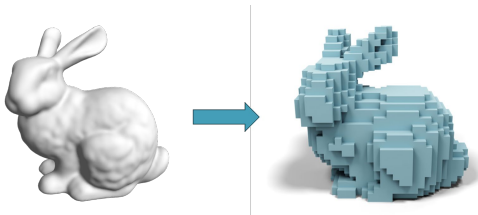
\includegraphics[width=0.6\linewidth]{imgs/lecture13/13.1 voxel representation.png}
        \caption{}
        \label{fig:13.1a}
    \end{subfigure}
    \hfill
    \begin{subfigure}[b]{0.45\textwidth}
        \centering
        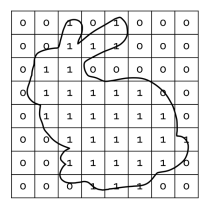
\includegraphics[width=0.4\linewidth]{imgs/lecture13/13.2 voxel representation.png}
        \caption{}
        \label{fig:13.1b}
    \end{subfigure}

    \caption{Voxel representation}
    \label{fig:13.1}
\end{figure}

\subsubsection{Point clouds}
Point clouds are unordered collections of point samples often originating from 3D scans. They are compact, easy to handle, and excellent for fast rendering of massive datasets or real-time tasks like autonomous driving. But, because they are just a collection of points, they are often irregular and do not truly represent a continuous surface.

\begin{figure}[htbp]
    \centering
    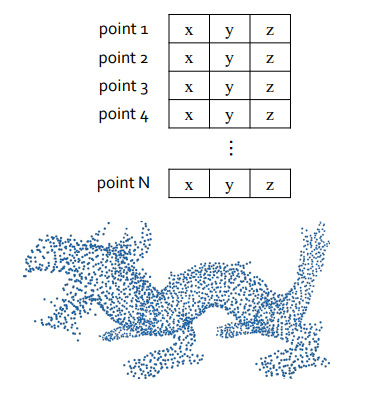
\includegraphics[width=0.4\linewidth]{imgs/lecture13/13.3 point cloud.png}
    \caption{Point cloud}
    \label{fig:13.2}
\end{figure}

\subsubsection{Triangle mesh}
The triangle meshes are the de facto standard for geometry processing. They represent a surface as a collection of triangles, which offers several advantages (Planarity and convexity, approximation power and so on). Every triangle is inherently flat and simple to calculate. \par
They are the most efficient way to store generic 3D surfaces for movies, video games, and 3D modeling. Unlike regular voxel grids, meshes can adapt their density, using many small triangles for detailed areas and fewer large ones for flat surfaces.

\section{Topological foundations}
To process geometric data accurately, computer graphics relies on topology to describe how elements are connected, regardless of their specific shape or position.

\begin{definition}[Simplice]
    The most basic building block used to construct a complex 3D shape is called a \emph{simplex}. A k-simplex is mathematically defined as the convex hull of h+1 affinely independent points, called vertices.
\end{definition}

There are four possible types of simplices: 0-simplex (a single point, a vertex); 1-simplex (a line segment connecting two points); 2-simplex (a triangle defined by three points); 4-simplex (a tetrahedron, a 3D pyramid shape defined by four points).

\begin{figure}
    \centering
    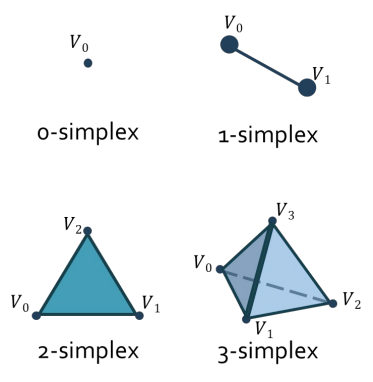
\includegraphics[width=0.35\linewidth]{imgs/lecture13/13.4 simplices.png}
    \caption{Simplices}
    \label{fig:13.3}
\end{figure}

\subsubsection{Faces and orientation}

\begin{definition}[Proper face]
    A proper face of a k-simplex (a simplex with k dimensions) is another simplex whose set of vertices is a non-empty proper subset of the vertices of the original simplex.
\end{definition}

In simpler terms, if you take some, but not all, of the points that define a shape and use them to form a new, lower-dimensional shape, that new shape is a proper face. For example, A 1-simplex (a line)'s proper faces are its two vertices (0-simplices); a 2-simplex(a triangle)'s proper faces are its three edges (1-simplices) and 3 vertices (0-simplices)

\subsubsection{Simplicial complexes}
A simplicial complex is a structured obtained by "gluing" the simplices. To be considered a proper complex, the collection must follow two rules:

\begin{itemize}[noitemsep]
    \item Any two simplices in the collection can only meet along a common face
    \item If a simplex is in the collection, all of its faces must also be included in the collection. 
\end{itemize}

The \textbf{dimension} of the simplicial complex is the maximum dimension of its simplices. A k-dimensional simplicial complex is homogeneous if it is made of k-simplices and their faces.

\begin{definition}[Homogeneity]
    A simplicial complex is called homogeneous if all its primary components are of the same dimension and do not have any dangling parts of lower dimension
\end{definition}

Under the definition of homogeneity, a triangle mesh is a homogeneous 2D simplicial complex because it is composed entirely of triangles and their shared edges and vertices.

\section{Topological relations}

\begin{definition}[Adjacency and incidency]
    Two k-simplices A and B are \emph{m-adjacent} (m<k) if there exists an m-simplex which is a proper face of both A and B (A and B share a common face).\par
    Two simplices are \emph{incident} if one is a proper face of the other
\end{definition}

For example, two triangles (2-simplices) sharing an edge (1-simplex) are 1-adjacent;  two triangles sharing a vertex (0-simplex) are 0-adjacent.\par
Two vertices (0-simplices) are adjacent if they are incident to a common edge (1-simplex).

\begin{definition}[Boundary]
    For a triangle mesh, the boundary is defined as the union of all edges that are incident to exactly one face. In a closed object with no holes, there is no boundary.
\end{definition}

\subsubsection{Manifoldness - Well-behaved surfaces}
Computer graphics often assumes surfaces are 2D manifolds, which is a way of saying they behave like physical, non-degenerate solids with no infinitely thin parts.\par
A continuous definition says that a surface is a manifold is every point on it has a neighborhood that can be continuously deformed into a disk.

\begin{figure}
    \centering
    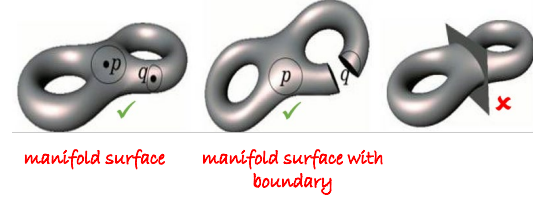
\includegraphics[width=0.5\linewidth]{imgs/lecture13/13.5 manifold.png}
    \caption{Manifoldness}
    \label{fig:13.4}
\end{figure}

On discrete rules for triangle meshes to be considered manifold, it must follow two specific rules:
\begin{itemize}[noitemsep]
    \item \textbf{Vertex rule}: the "star" (the collection of triangles surrounding a vertex) must form a single connected "fan". You must be able to travel between any two triangles in the star without leaving the neighborhood 
    \item \textbf{Edge rule}: every edge must be incident to at least two faces(one for a boundary, two for an interior).
\end{itemize}

\begin{figure}
    \centering
    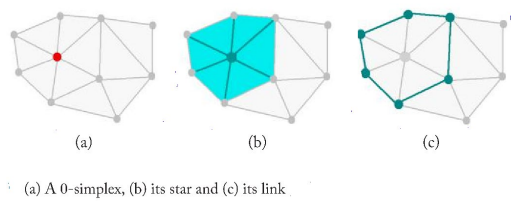
\includegraphics[width=0.5\linewidth]{imgs/lecture13/13.6 star and link.png}
    \caption{Star and link}
    \label{fig:13.5}
\end{figure}

In the fig.\ref{fig:13.5}, the simplex in question is a vertex (0-simplex), and its "\textbf{star}" is the union of all the simplices containing the said vertex forming the figure b. Its \textbf{link} is all the faces of the simplices in the star of the vertex that do not intersect with it. 

\subsection{Normals on meshes}
Normals (vectors perpendicular to the surface) are critical for tasks like shading.\par
In a continuous mathematical model, the unit surface normal vector at a specific point p is the vector that is orthogonal to the tangent plane at that point. This tangent plane is spanned by the tangent vectors to curves passing through p, and is calculated using the partial derivatives of a regular surface parametrization.\par
In the discrete case, because triangle meshes are discrete collections of flat faces, evaluating normals requires a different approach. Because the triangles are perfectly flat (planar), their normals are constant and easily calculated using the cross product of two edges. \par
To get a smooth look across a jagged mesh (such as in Gouraud or Phong shading), normals must be evaluated at the vertices. The standard is to compute the vertex normal as a weighted average of the normals of all triangles in its star. Using constant weights can be counterintuitive on irregular meshes, so weighting by triangle area or angle is preferred for better results. 
\chapter{Lecture 14 - Rendering}
\begin{definition}[Rendering]
    \emph{Rendering} is the process of converting input data, such as 3D geometry and material properties, into a final image. To visualize a 3D scene, it must be transformed into a synthetic raster image that can be displayed on a screen.
\end{definition}

To render a scene effectively, an algorithm requires several types of input: \textit{geometric data} (the raw shapes of the objects), \textit{material and texture} (information about how surfaces look and react to light), a \textit{synthetic scene} (the arrangement of these objects in a virtual space), \textit{camera model} (a mathematical description of the "picture-making apparatus").\par
The material categorizes rendering into three families of algorithms:
\begin{itemize}[noitemsep]
    \item \textit{Ray tracing}: tracing the path of light to simulate visual effects
    \item \textit{Path tracing}: a specialized, more advanced form of ray tracing
    \item \textit{Rasterization-based pipeline}: the standard approach for real-time graphics, which converts 3D primitives directly into 2D pixels
\end{itemize}

\subsubsection{The Pinhole camera}
The pinhole camera is a fundamental mathematical model used in computer graphics as a metaphor for the virtual camera, describing the relationship between an observer and a 3D scene.\par
It is modeled as a parallelepiped (a box) where the front face contains an infinitesimally small hole. When the light enters through this hole, the resulting image is formed on the back side of the box, known as the focal plane. \par
This pinhole camera is formed of components: the \textit{viewpoint} is the eye position or the projection center located at the pinhole itself; the \textit{focal distance} (\textit{d}) is the distance between the pinhole (projection center) and the back side of the box where the image forms; while a physical pinhole camera forms an inverted image on the back of the box, computer graphics conventions often assume the existence of an image plane located between the scene and the projection center to simplify calculations.\par
The model allows for precise control over what is visible in the rendered scene. The angle of view \(\theta\) can be controlled by varying the ratio between the focal distance \textit{d} and the height of the image plane \textit{h}.

\begin{figure}[htbp]
    \centering
    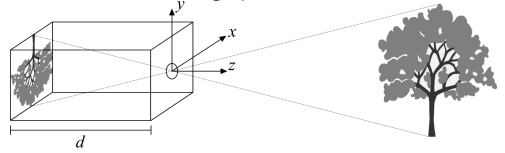
\includegraphics[width=0.5\linewidth]{imgs/lecture14/14.1 pinhole camera.png}
    \caption{Pinhole camera}
    \label{fig:14.1}
\end{figure}

\section{The chain of transformations}
\begin{definition}[chain of transformations]
    The chain of transformations is the technical process of transforming 3D models into 2D synthetic scenes through a sequence of mathematical mappings. 
\end{definition}

\begin{figure}[htbp]
    \centering
    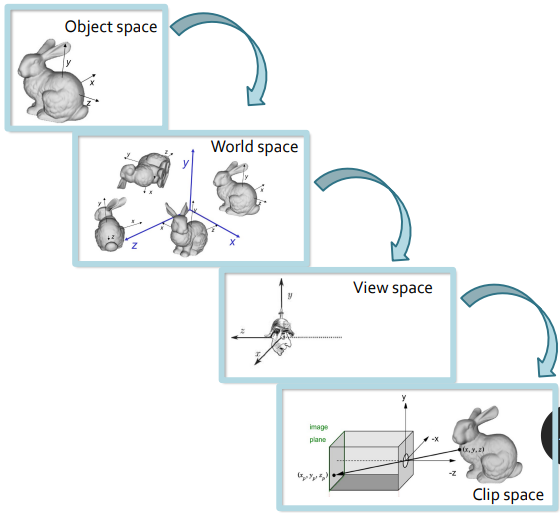
\includegraphics[width=0.4\linewidth]{imgs/lecture14/14.2 chain of transformations.png}
    \caption{The chain of transformations}
    \label{fig:14.2}
\end{figure}

This chain of transformations requires the definition and computation of proper transformations. The hierarchy of space is the following:
\begin{itemize}[noitemsep]
    \item \textbf{Object space} (local space): this is the reference frame where a 3D model is originally defined. Each object has its own space, arbitrarily chosen by the modeler to define its specific point coordinates and normals 
    \item \textbf{World space}: because a scene contains many different models, a common reference system is needed to arrange them; this is the world space. The \textbf{modeling transformation} maps an object from its local space into this shared world space, defining its position, rotation, and scale within the scene
    \item \textbf{View space} (camera/eye space): this space has its origin at the camera center. A second transformation moves objects from the world space into the view space so that their coordinates are relative to where the "eye" sees
    \item \textbf{Clip space}: this is the final destination, aligned with the 2D screen of the output device. Mapping to this space involves projecting 3D elements onto a 2D plane
\end{itemize}

\subsection{Affine transformations}
\begin{definition}[Affine transformations]
    In Euclidean geometry, an affine geometry is a geometric transformation that preserves lines and parallelism.
\end{definition}
We need transformations to translate, scale, rotate, and deform 3D objects, to go from the object to the world space. These transformations are called affine.\par
The affine transformations send points to points, lines to lines, planes to planes, and so on, while \textit { maintaining the ratios of distances} between points on a straight line (midpoint of a segment goes to midpoint of a segment). However, affine transformations do not necessarily preserve angles between lines or distances between points. Examples of affine transformations include translation, rotation, scaling, shear, reflection, and compositions of them in any sequence.

\subsection{Composing transformations}
Often, multiple transformations (like rotating an object and then translating it) need to be combined. The problem is that while rotation and scaling are expressed as products (multiplication), translation is expressed as a sum, making them difficult to combine into a single operation.\par
A possible solution is to use the so-called homogeneous coordinates, that is, a different representation for points and vectors that adds an extra dimension with respect to Cartesian coordinates (a third coordinate w for 2D, or a fourth for 3D).

\subsubsection{Homogeneous coordinates}
Given a 2D point P(x, y) is represented as (\(x_h, y_h, w\)), with \(w \neq 0\). To convert back to original Cartesian coordinates, you divide by the extra dimension: \(x = x_h/w \ and \ y = y_h/w\). By convention, w is usually set to 1 for specific locations (x, y, 1).\par
A big advantage in using this system is that, all affine transformations, including translation, can be represented as \(3 \times 3 \) matrices (for 2D) or \(4 \times 4\) matrices (for 3D). This facilitates the mathematical concatenation of several transformations into one by simply multiplying the matrices. This results in a single "master matrix" that can be applied to every point in a 3D model in one step. \par
We can also use homogeneous coordinates to remove points/vectors ambiguity, by setting w coordinates to 1, we have points (locations); and when w = 1, we have vectors (directions) representing "points at infinity".

\section{Ray tracing}
\begin{definition}
    Ray tracing is a rendering paradigm that simulates the way light behaves in the real world by following its path.
\end{definition}
The main idea of the ray tracing is tracing backwards. In nature, light rays travel from a source, bounce off objects, and eventually enters our eyes. Because the vast majority of light rays in a scene never reach the observer, simulating all of them would be a vast amount of energy. So, instead of tracing light from the source, ray tracing works backward. For each pixel on the screen, the algorithm shoots a ray, called a \textbf{primary ray}, from the viewpoint into the scene. And the algorithm finds where that ray intersects with the closest primitive (object) in the 3D scene. The color of that pixel is then determined by the properties of the object hit at that specific point. \par

\subsubsection{Secondary rays}
One of the primary advantages of ray tracing is that it handles complex optical phenomena "naturally" through the use of secondary rays:
\begin{itemize}[noitemsep]
    \item To see if a point is in shadow, the algorithm shoots a "\textbf{shadowing ray}" from the intersection point toward the light source. If it hits an object on the way, the point is in shadow.
    \item If the ray hits a mirror-like surface, a new "\textbf{reflection ray}" is bounced off the surface to see what other objects are reflected in it.
    \item For semi-transparent objects like glass or water, the algorithm calculates a "\textbf{refracted ray}" that passes through the material, allowing for a realistic simulation of transparency.
\end{itemize}

\begin{figure}[htbp]
    \centering
    
    \begin{subfigure}[b]{0.45\textwidth}
        \centering
        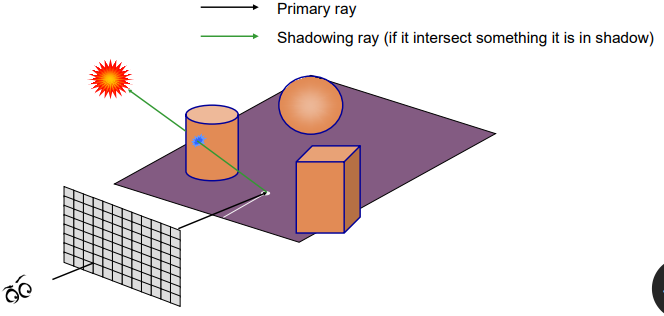
\includegraphics[width=0.8\linewidth]{imgs/lecture14/14.3 ray tracing and shadow ray.png}
        \caption{Shadowing ray}
        \label{fig:14.3a}
    \end{subfigure}
    \hfill
    \begin{subfigure}[b]{0.45\textwidth}
        \centering
        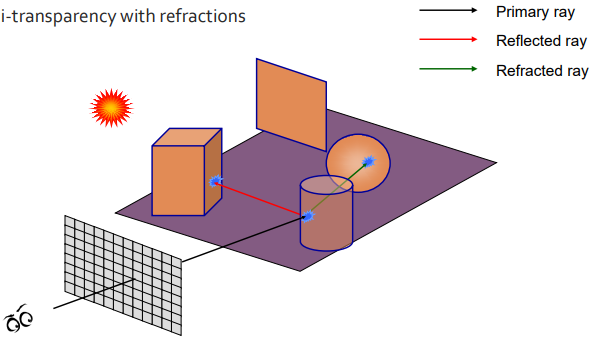
\includegraphics[width=0.8\linewidth]{imgs/lecture14/14.4 ray tracing and reflectio refraction ray.png}
        \caption{Reflection and refraction rays}
        \label{fig:14.3b}
    \end{subfigure}

    \caption{Ray tracing: primary and secondary rays}
    \label{fig:14.3}
\end{figure}

\subsubsection{Primitives and geometry}
Ray tracing offers more freedom in the types of shades it can render compared to other methods. While most real-time systems rely on triangles, ray tracing can intersect rays with any mathematical primitive that has a defined intersection formula, including spheres, implicit surfaces, and Geometric Solid Modeling (GSM).

\subsubsection{Computational cost}
Historically, ray tracing was considered "too slow" for real-time use because the core operation, computing the intersection between a 3D ray and 3D primitives, is complex. However, the cost is actually sublinear relative to the number of objects in the scene, provided the right data structures are used. And to speed up calculations, spatial indexing is used, a specialized hierarchical or hashing-based data structures that allow the algorithm to quickly skip parts of the scene the ray won't hit.\par
Modern GPUs, like NVIDIA RTX, now combine ray tracing with traditional methods to achieve the effects in real-time.

\section{Rasterization}
Rasterization is the alternative to ray tracing, which is the standard method for real-time graphics. While ray tracing works by shooting rays from the observer for each pixel, rasterization takes the opposite approach: \textbf{it takes each 3D object and determines which pixels it covers on the screen}.
\begin{definition}[Rasterization]
    Rasterization is a rendering paradigm that converts 3D geometric data into a 2D raster image by determining which pixels on the screen are covered by each 3D object.
\end{definition}

Because modern GPUs are highly optimized for rasterization, almost every 3D scene is decomposed entirely into triangles before being rendered. Rasterization is also frequently called the \textbf{T \& L pipeline}, consisting of two primary computational goals:
\begin{itemize}[noitemsep]
    \item \textbf{Transform}: the algorithm projects 3D primitives (geometric shapes) from their world coordinates into the 2D "screen space" of the output device
    \item \textbf{Lighting}: the algorithm computes the final color for every part of the scene, taking into account the geometry, the light sources, and the optical characteristics of the material
\end{itemize}

\subsubsection{Rasterization process}
The process flows through four distinct stages to turn a vertex into a pixel:
\begin{enumerate}[noitemsep]
    \item Per-vertex transformations: individual vertices and their attributes are moved into the correct coordinate spaces
    \item Primitive processing: the vertices are assembled into basic shapes, while points and lines are possible, triangles are the universal standard because graphics HW is specifically optimized to process them
    \item Rasterization: the core step where a 2D shape on the screen is filled with a grid of fragments. A fragment is essentially a "potential pixel" that carries all the data necessary to compute a final color.
    \item Per-fragment computation: the final color of each fragment is determined, often by accessing texture RAM to apply images to the surface, before the results are written to the frame buffer.
\end{enumerate}

\subsubsection{Attributes Interpolation and Perspective correction}
During rasterization, the values defined at the corners of the triangle, the vertices, must be spread across the entire surface. If  \textit{Barycentric coordinates} are used, the algorithm performs a linear interpolation of attributes like colors or normals across the face of a triangle. If \textit{Perspective correction} is used, a simple linear interpolation of texture coordinates across a triangle can cause visual distortion due to the way perspective works. Rasterization HW must apply a perspective correction formula using the depth (w) coordinate to ensure textures appear correctly aligned as they recede into the distance.

\begin{figure}
    \centering
    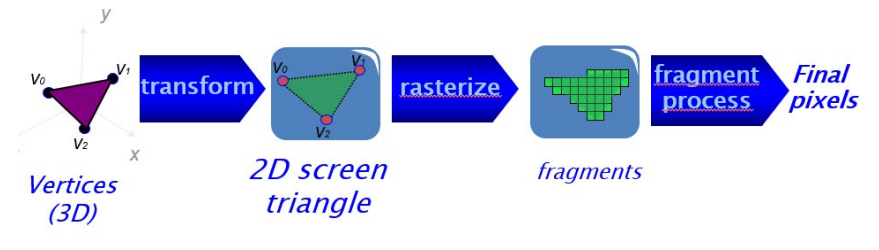
\includegraphics[width=0.5\linewidth]{imgs/lecture14/14.5 rasterization pipeline.png}
    \caption{Rasterization-based rendering}
    \label{fig:14.4}
\end{figure}
\subsubsection{Advantages and limitation}
Rasterization remains the dominant paradigm despite the rise of ray tracing, thanks to the ease of \textbf{parallelism}, making it perfectly suited for the architecture of modern GPUs; the high \textbf{scalability} of image resolution, meaning increasing the number of pixels on a screen has a more predictable performance cost than in ray tracing. \par
However, a historical disadvantage of rasterization is that it cannot naturally handle "global" effects like shadows or reflections. But designers have developed "clever" advanced algorithms to approximate these effects with compromise-level quality in real-time.

\section{Ray tracing Vs Rasterization}
The debate between ray tracing and rasterization stems from their fundamentally different approaches to generating an image from 3D data. It is a choice between processing the scene "pixel by pixel" Vs "primitive by primitive".\par
Quick recap, in ray tracing, for each pixel on the screen, the algorithm checks every geometric primitive in the screen to see if it is hit by a ray; in rasterization, for each geometric primitive (usually a triangle), the algorithm determines which pixels on the screen it covers.

\subsubsection{Advantages of \textit{Ray tracing}}
Ray tracing is often preferred for high-fidelity, "off-line" rendering, such as in movies by Pixar or DreamWorks, for several reasons:
\begin{itemize}[noitemsep]
    \item \textbf{Global effects} --> it naturally handles complex optical phenomena like shadows, specular reflections, and refractions
    \item \textbf{Conceptual simplicity }--> the underlying algorithm is straightforward, you simply trace the path of light
    \item \textbf{Primitive freedom} --> it is easier to calculate the intersection of a ray with complex mathematical shapes (spheres, implicit surfaces) than it is to project and fill those shapes as pixels
    \item \textbf{Scene scalability} --> if a specialized data structure for "spatial indexing" is used, the computational cost can be sublinear relative to the number of objects in the scene
\end{itemize}

\subsubsection{Advantages of \textit{Rasterization}}
Rasterization is the standard for "real-time" rendering, such as video games and web previews, because of its efficiency:
\begin{itemize}[noitemsep]
    \item \textbf{Parallelism and HW optimization} --> the algorithm is easily parallelizable and was the first to receive specialized HW support, GPUs
    \item \textbf{Resolution scalability} --> it scaled better with image resolution (the number of pixels) than ray tracing
    \item \textbf{Handling dynamic data} --> it is generally easier to manage scenes where objects are constantly moving
    \item \textbf{Speed} --> it is inherently fast because it only processes the specific pixels covered by a primitive rather than checking every primitive for every pixel
\end{itemize}

\subsubsection{The reality of the debate...}
The traditional boundaries between these two methods are blurring. The current state is that \textit{rasterization is fast, but needs cleverness to support complex visual effects; ray tracing supports complex visual effects, but needs cleverness to be fast}.\par
A clever rasterization utilizes real-time engines that use algorithms and approximations to simulate the reflections and shadows that ray tracing produces naturally. While clever ray tracing uses efficient spatial queries to avoid being slow. \par
Modern technology, such as NVIDIA RTX, has effectively ended the binary debate by combining both rasterization and ray tracing within the same HW to achieve high-quality visual effects at real-time speeds.
\chapter{Lecture 15 - Lighting}
Lighting can be perceived and mathematically modeled in different ways:
\begin{itemize}[noitemsep]
    \item \textit{Ray optics}: the light is modeled using rays. The rays follow geometric rules, which can model several lighting effects like reflection and refraction
    \item \textit{Wave optics}: the light is modeled as a propagating wave, which can model lighting effects such as diffraction
    \item \textit{Electromagnetic optics}: it can describe lighting effects like the polarization of the light, not explained by the wave optics
    \item \textit{Photon optics}: quantum mechanics is used to model lighting effects
\end{itemize}

The lighting is a process where energy is emitted from a source (like a lamp or the sun), travels through a scene, and interacts with objects until it stabilizes. This happened at the speed of light, making the result appear instantaneous and table to the human eye.\par
When a ray of light hits a surface, several effects happen simultaneously: specular reflection (light bounced off in a specific direction, like a mirror), diffusion (light scatters in many directions), transmission (light passes through the material, refraction), absorption (the material soaks up the energy), and scattering/emission (effects like fluorescence).

\subsubsection{Solid angle}
To calculate lighting in 3D space, the solid angle (\(\Omega\)) is introduced, which is the 3D extension of a 2D planar angle. It represents the angular dimension of a cone pointing in a specific direction. It is measured in steradians (sr). A full hemisphere corresponds to a solid angle of \(2\pi\) steradians.

\begin{figure}[htbp]
    \centering
    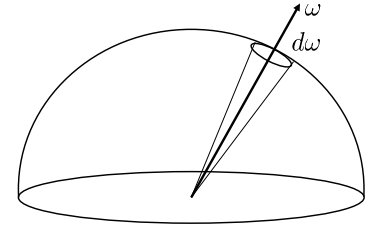
\includegraphics[width=0.3\linewidth]{imgs/lecture15/15.1 solid angle.png}
    \caption{Solid angle}
    \label{fig:15.1}
\end{figure}

\subsubsection{Radiometry}
Radiometry defines three critical units used to quantify light in a scene:
\begin{itemize}[noitemsep]
    \item Radiant flux \(\Phi\), measured in Watts, this is the total radiant energy passing through a surface per unit of time
    \item Irradiance \(E\), the radiant flux incident on a specific surface element (\(Watts/m^2\))
    \item Radiance \(L\), the radiant flux per solid angle per unit area (\(Watts/m^2sr\)). This is effectively what a camera or an eye "sees" from a specific direction
\end{itemize}

A fundamental takeaway is that for a point light source emitting light uniformly in all directions, \textit{the intensity (irradiance) reduces with the square of distance} (\(1/r^2\)).

\section{Rendering equation}
\begin{definition}[Rendering equation]
    The rendering equation is the fundamental formula for calculating the total visible light (\(L_o\)) at any point on a surface from a specific direction. 
\end{definition}

The rendering equations calculate the visible light in a point of the scene for a specific direction, given by the sum of emitted light and the light reflected in that direction: \textit{emitted light} (\(L_e\)), which is the energy the object produces itself; and \textit{reflected light} (\(L_r\)), which is the light from the environment that bounces off the surface. To find the reflected light, the algorithm must integrate all incoming light contributions from every direction in the hemisphere above the point, weighting them according to the material's properties and the angle of reflection.\par
There are two specialized functions to mathematically represent how different surfaces (wood, metal, skin ..) look; these two are BSSRDF and BRDF

\subsubsection{BSSRDF}
Bidirectional Scattering Surface Reflectance Distribution Function.\par
The function describes the most general case of light-material interaction, where light hits a surface and may leave from a different position; the process is called scattering.

\subsubsection{BRDF}
Bidirectional Reflectance Distribution Function.\par
Because of the complexity of BSSRDF, computer graphics often uses the BRDF as an approximation. It assumes light enters and leaves at the same point x. It is defined as the ratio between the outgoing radiance (reflected light) in a certain direction and the incident irradiance (incoming light) from another direction.

\section{Local lighting model}
Because calculating the full rendering equation is computationally too expensive for real-time systems, designers use local lighting models to approximate the way light interacts with surfaces. These models focus only on the local effects, ignoring the complex "global" inter-reflection between all objects in a scene.

\begin{definition}[Global effects]
    Global effects involve interactions between multiple objects, such as soft shadow, indirect lighting (color bleeding), and caustics
\end{definition}

\begin{definition}[Local effects]
    Local lighting models simplify the scene by calculating light for a single point based only on its own properties and the direct light sources, ignoring reflections from other objects.
\end{definition}

\subsection{Phong lighting model}
The Phong model is a fundamental tool for simulating how \textit{opaque} materials look under a point light source. While it is quite realistic, the sources note that some materials can end up looking like plastic. It simplifies the math by breaking the final color into three distinct components:
\begin{itemize}[noitemsep]
    \item \textbf{Ambient component}: this term is used to \textit{roughly approximate global inter-reflections}. It provides a constant base level of light to all points in the scene so that areas not directly hit by a light source are not completely black
    \item \textbf{Diffuse components}: based on Lambert's law, this represents \textit{light that hits a rough surface} (like wood or stone) and reflects uniformly in all directions. The intensity depends on the angle (\(\theta\)) between the light source and the surface normal; it is brightest when the light is directly overhead
    \item \textbf{Specular component}: this models the "shiny" part of an object, the specular highlight. It \textit{simulates light reflection off smooth, mirror-like surfaces} in a specific direction. Unlike diffuse light, the appearance of the specular highlight depends on the position of the observer.
\end{itemize}

A critical part of the specular term is the exponent (n). This parameter defines how "sharp" or "focused" the specular highlight is. A high value of n creates a very small, bright portion of light (like a polished billiard ball), while a lower value makes the highlight larger and more spread out.\par
The model also accounts for light attenuation, where the intensity of the light source decreases as the distance (\(d_L\)) from the light to the surface increases.

\section{Shading}
\begin{definition}
    Shading is the process of computing the actual color of each pixel on the screen based on the lighting models. It determines where and how often the light-material interactions are calculated on a 3D model
\end{definition}
There are three primary types of shading: Flat shading, Gouraud shading, and Phong shading.

\subsubsection{Flat shading}
Flat shading is the simplest form of shading, where the lighting equation is computed only once for each face (polygon) of the 3D model. In which the algorithm uses the face normal to determine a single color, which is then applied uniformly across the entire surface of that face. \par
Because each face has a single solid color, the edges between them become very obvious, and the object looks "blocky." Even if you use a massive number of faces to try to smooth the object, it will fail to smooth the edges.

\begin{figure}[htbp]
    \centering
    \includegraphics[width=0.5\linewidth]{imgs/lecture15/15.2  flat shading.png}
    \caption{On the left, the flat shading, on the right, the reference object}
    \label{fig:15.2}
\end{figure}

The visual effect of \textbf{Mach Banding} is the perceptual phenomenon where the human eye exaggerates the contrast at the borders between different shades, making discontinuities clearly visible, thus explaining the presence of "blocky" edges.

\begin{figure}[htbp]
    \centering
    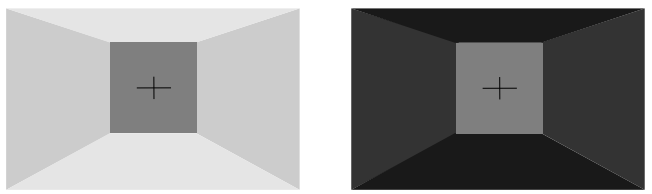
\includegraphics[width=0.5\linewidth]{imgs/lecture15/15.3 mach banding.png}
    \caption{Mach Banding}
    \label{fig:15.3}
\end{figure}

\subsection{Gouraud shading}
To fix the blockiness of flat shading, Gouraud shading calculates the lighting at the vertices instead of the faces. The lighting equation is computed for each vertex using a vertex normal (often calculated as the average of the normals of the faces meeting at that vertex). The colors at the vertices are then linearly interpolated across the face of the triangle during rasterization. This creates a much smoother appearance, making faceted models look like continuous curved surfaces.\par
But, it struggles with specular highlights. If a highlight (the bright, shiny spot) falls in the middle of a face rather than near the vertex, it might be missed entirely or appear distorted because the interpolation only knows about the colors at the corners. It can also have visual issues at the corners of objects.

\subsection{Phong shading}
Phong shading provides the highest quality results by moving the lighting calculation from the vertices to the individual pixels (fragments). Instead of interpolating the colors from the vertices, this method interpolates the surface normals across the face of the triangle. The lighting equation is then computed for every single pixel using these interpolated normals.\par
This is the most realistic method out of the three. It correctly renders specular highlights even if they are very small or fall in the center of a face, and it provides a perfectly smooth appearance for curved surfaces.

\begin{figure}[htbp]
    \centering
    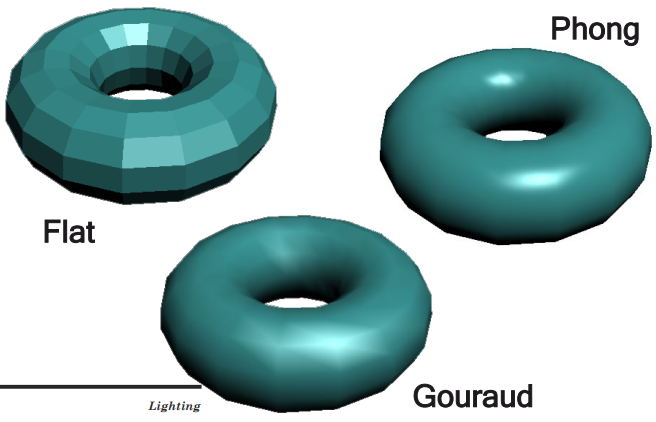
\includegraphics[width=0.5\linewidth]{imgs/lecture15/15.4 shading.png}
    \caption{Shading methods result comparison}
    \label{fig:15.4}
\end{figure}
\chapter{Lecture 16 - Texture}
Texturing is a fundamental technology in computer graphics used to add high levels of visual detail to 3D surfaces without requiring complex geometric modeling.

\begin{definition}
    Texturing is the process of modulating the attributes of vertices, such as color, normals, or transparency, to obtain a specific visual effect.
\end{definition}

During rendering, textures are stored in a specialized memory on the graphics card called Texture RAM. Each texture is a 1D, 2D, or 3D array of \textbf{texels} of the same data type (a texel is the base element, just like a picture is made of pixels). Depending on what the texel represents, a texture can be a color map (RGB), an alpha map (transparency), a normal map (surface orientation: X, Y, Z), or a shininess map (specular coefficients).

The most common form of texturing is \textbf{texture mapping}, where the color attribute is modulated to wrap a 2D image around a 3D object.\par
To tell the computer how to wrap the image, every vertex in a 3D model is assigned coordinates in a 2D "texture space", also known as \textbf{uv space}.

\subsection{UV space}
Every vertex in a 3D mesh is assigned a coordinate (x, v) ranging from 0.0 to 1.0, which corresponds to a specific location on the 2D texture image. During rasterization, these u, v coordinates are interpolated across the face of a triangle so the system knows which part of the image belongs to which pixel. \par
These u, v coordinates can be assigned manually during modeling, precomputed, or generated automatically using projection functions. Different techniques of texture coordinates assignment need to be uses to speed up the texture transfer CPU RAM - Texture RAM. The specific technique to be used depends on the application.\par

\begin{figure}[htbp]
    \centering
    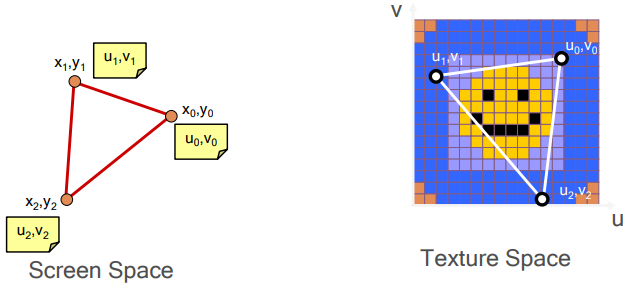
\includegraphics[width=0.5\linewidth]{imgs/lecture16/16.1.png}
    \caption{UV Space}
    \label{fig:16.1}
\end{figure}

Attribute interpolation using Barycentric coordinates and perspective correction is also used here in texturing.

\begin{figure}[htbp]
    \centering
    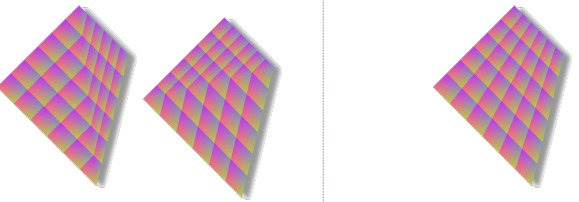
\includegraphics[width=0.4\linewidth]{imgs/lecture16/16.2 attribute interpolation.png}
    \caption{Left without interpolation, right with interpolation}
    \label{fig:16.2}
\end{figure}

\subsection{Texture look up}
When a pixel on the screen does not perfectly align with a texel in the image, the system must perform a texture look-up using filtering techniques:
\begin{itemize}[noitemsep]
    \item \textbf{Magnification} is used when a pixel is larger than a texel. To avoid a "blocky" look, the system uses \textit{nearest filtering} (choosing the closest texel) or \textit{bilinear interpolation} (averaging the closest texels for a smoother look)
    \item \textbf{Minification} is used when a pixel is smaller than a texel. This often causes visual artifacts like aliasing. The standard solution is \textit{mip-mapping}, where the system pre-computes several lower-resolution versions of the texture and chooses the one that best matches the current viewing distance.
\end{itemize}

\begin{figure}[htbp]
    \centering
    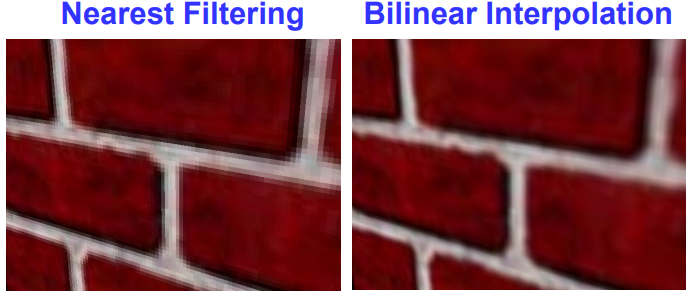
\includegraphics[width=0.3\linewidth]{imgs/lecture16/16.4 magnification.png}
    \caption{Magnification methods comparison}
    \label{fig:16.3}
\end{figure}

\begin{figure}[htbp]
    \centering
    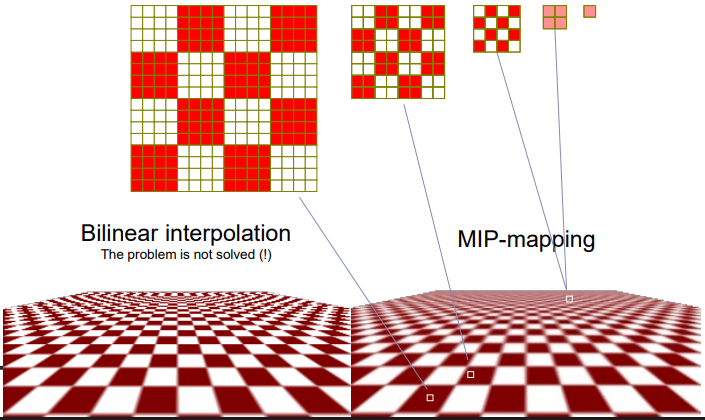
\includegraphics[width=0.5\linewidth]{imgs/lecture16/16.3 mip-mapping.png}
    \caption{Mip-mapping visualized}
    \label{fig:16.4}
\end{figure}

If a vertex is assigned texture coordinates outside the standard range, the system uses one of two modes: 
\begin{itemize}[noitemsep]
    \item \textbf{Clamp mode}, any coordinate less than 0 is treated as 0, and anything greater than 1 is treated as 1, effectively stretching the edge texels
    \item \textbf{Repeat mode}, the integer part of the coordinate is ignored, causing the texture to tile across the surface, which is highly efficient for larger surfaces like brick walls.
\end{itemize}

\subsection{Advanced mapping techniques}
Building on the standard color modulation of texture mapping, the following advanced mapping techniques designed to simulate complex optical effects and intricate surface details. 

\subsubsection{Environmental mapping}
The environmental mapping is used to simulate an object reflecting its surroundings without the high computational cost of full ray tracing. A texture, known as an environment map, captures the colors of the reflected scene. There are two primary methods for applying this:
\begin{itemize}[noitemsep]
    \item \textbf{Sphere mapping}: the technique maps the environment onto a virtual sphere surrounding the object. It uses spherical coordinates derived from the reflection vector to determine which part of the environment is visible from the observer's viewpoint.
    \item \textbf{Cube mapping}: this is often preferred because it provides more uniform sampling than sphere mapping and is easier to generate. The environment is projected onto the six faces of a virtual cube. 
\end{itemize}

\subsubsection{Bump mapping}
Bump mapping is introduced as a way to simulate surface irregularities like wrinkles or bumps. Bump mapping alters the way light hits a surface without modifying its actual 3D geometry. The technique uses a texture (a normal map) to perturb the surface normals of an object. Because lighting calculations depend heavily on surface normals, the light "tricks" the eye into seeing depth and texture on a perfectly flat surface. However, because the geometry is unchanged, the silhouette of the object remains perfectly smooth.

\subsubsection{Displacement mapping}
Displacement mapping is a more advanced alternative to bump mapping that provides a much higher level of realism. Unlike bump mapping, this technique effectively moves the 3D points of the surface during rendering. Because the geometry itself is moved, the silhouette of the model is correctly deformed. This allows for the realistic rendering of very rough surfaces, such as jagged rocks or heavy cratering, that bump mapping cannot convincingly simulate. 

\begin{figure}[htbp]
    \centering
    
    % First row
    \begin{subfigure}{0.45\textwidth}
        \centering
        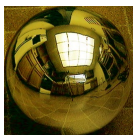
\includegraphics[width=0.4\linewidth]{imgs/lecture16/16.5 sphere mapping.png}
        \caption{Sphere mapping example}
        \label{fig:16.5a}
    \end{subfigure}
    \hfill
    \begin{subfigure}{0.45\textwidth}
        \centering
        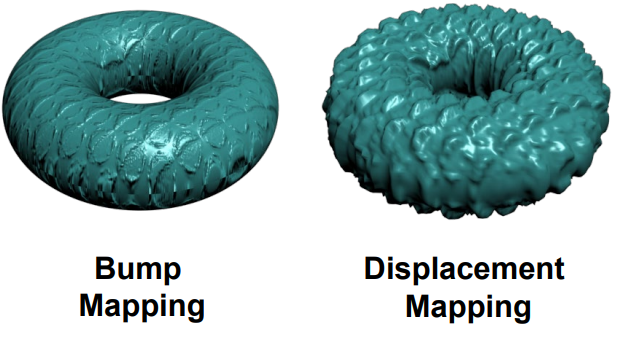
\includegraphics[width=0.8\linewidth]{imgs/lecture16/16.7 bump and displacement mapping.png}
        \caption{Bump mapping and displacement mapping examples}
        \label{fig:16.5b}
    \end{subfigure}

    \vspace{0.5cm}

    % Second row 
    \begin{subfigure}{\textwidth}
        \centering
        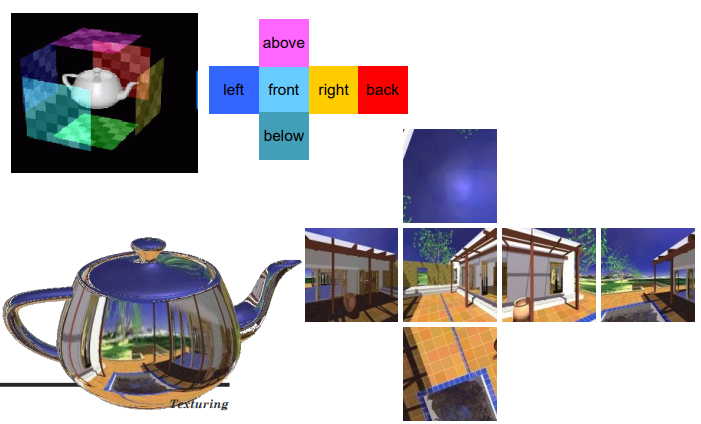
\includegraphics[width=0.7\linewidth]{imgs/lecture16/16.6 cube mapping.png}
        \caption{Cube mapping example}
        \label{fig:16.5c}
    \end{subfigure}

    \caption{Texture techniques}
    \label{fig:16.5}
\end{figure}
\include{lectures/lecture17}

\end{document}